%% 
%% Copyright 2007-2024 Elsevier Ltd
%% 
%% This file is part of the 'Elsarticle Bundle'.
%% ---------------------------------------------
%% 
%% It may be distributed under the conditions of the LaTeX Project Public
%% License, either version 1.3 of this license or (at your option) any
%% later version.  The latest version of this license is in
%%    http://www.latex-project.org/lppl.txt
%% and version 1.3 or later is part of all distributions of LaTeX
%% version 1999/12/01 or later.
%% 
%% The list of all files belonging to the 'Elsarticle Bundle' is
%% given in the file `manifest.txt'.
%% 
%% Template article for Elsevier's document class `elsarticle'
%% with numbered style bibliographic references
%% SP 2008/03/01
%% $Id: elsarticle-template-num.tex 249 2024-04-06 10:51:24Z rishi $
%%
% \documentclass[preprint,12pt,draft]{elsarticle}

%% Use the option review to obtain double line spacing
%% \documentclass[authoryear,preprint,review,12pt]{elsarticle}

%% Use the options 1p,twocolumn; 3p; 3p,twocolumn; 5p; or 5p,twocolumn
%% for a journal layout:
% \documentclass[draft,1p,times]{elsarticle}
% \documentclass[final,1p,times,sort&compress]{elsarticle}
% \documentclass[final,1p,times,twocolumn]{elsarticle}
\documentclass[final,3p,times,sort&compress]{elsarticle}
%% \documentclass[final,3p,times,twocolumn]{elsarticle}
% \documentclass[final,5p,times]{elsarticle}
% \documentclass[final,5p,times,twocolumn]{elsarticle}

%% For including figures, graphicx.sty has been loaded in
%% elsarticle.cls. If you prefer to use the old commands
%% please give \usepackage{epsfig}
%% 主要数学宏包
\usepackage{amsmath}     % 数学公式环境
\usepackage{amssymb}     % 提供 \mathbb 等数学符号
\usepackage{stmaryrd}    % 提供额外的数学符号
\usepackage{mathrsfs}    % 提供花体字母
\usepackage{tabularx}    % 可调列宽的表格
\usepackage{array}       % 提供高级列格式功能}
%% 图形、表格相关宏包
\usepackage{graphicx}    % 插入图像
\usepackage{caption}     % 修改图表标题
\usepackage{subcaption}  % 子图功能
\usepackage{multirow}    % 表格中单元格合并功能
\usepackage{booktabs}    % 提供 \toprule, \midrule, \bottomrule
\usepackage{tabularx}    % 可调列宽的表格
\usepackage{array}       % 提供高级列格式功能
\usepackage{float}       % 提供 [H] 位置选项
% \usepackage{XeCJK}       % 提供中文支持
%% 参考文献、链接相关宏包
\usepackage{hyperref}    % 创建可点击的交叉引用和链接
\hypersetup{             % 超链接设置
    colorlinks=true,
    linkcolor=blue,
    citecolor=blue,
    filecolor=magenta,      
    urlcolor=blue,
}

% 注意：cleveref 宏包必须放在 hyperref 宏包的【后面】加载！
\usepackage[capitalize,nameinlink]{cleveref}

%% 排版和图文混排
\usepackage{wrapfig}     % 实现图文并排，将图片排版在文字右边

%% 颜色和样式
\usepackage{xcolor}      % 提供颜色支持

%% 算法相关宏包
\usepackage{algorithm}   % 算法环境
\usepackage{algorithmic} % 算法的伪代码支持

%% 可选宏包（根据需求决定是否使用）
% \usepackage{amsthm}     % 提供定理环境

%% The lineno packages adds line numbers. Start line numbering with
%% \begin{linenumbers}, end it with \end{linenumbers}. Or switch it on
%% for the whole article with \linenumbers.
\usepackage{lineno}

\journal{Nuclear Engineering and Technology}
% \journal{J. Comput. Phys.}
% \journal{Nat. Comput. Sci.}
% \journal{Comput. Methods Appl. Mech. Eng.}

\begin{document}
\linenumbers
\begin{frontmatter}

    %% Title, authors and addresses

    %% use the tnoteref command within \title for footnotes;
    %% use the tnotetext command for theassociated footnote;
    %% use the fnref command within \author or \affiliation for footnotes;
    %% use the fntext command for theassociated footnote;
    %% use the corref command within \author for corresponding author footnotes;
    %% use the cortext command for theassociated footnote;
    %% use the ead command for the email address,
    %% and the form \ead[url] for the home page:
    %% \title{Title\tnoteref{label1}}
    %% \tnotetext[label1]{}
    %% \author{Name\corref{cor1}\fnref{label2}}
    %% \ead{email address}
    %% \ead[url]{home page}
    %% \fntext[label2]{}
    %% \cortext[cor1]{}
    %% \affiliation{organization={},
    %%             addressline={},
    %%             city={},
    %%             postcode={},
    %%             state={},
    %%             country={}}
    %% \fntext[label3]{}

%    \title{A deep learning method based on variable-domain integral weak solutions for neutron diffusion calculations in heterogeneous media}
    % \title{A variable-domain integral weak solution deep learning method for neutron diffusion calculations in heterogeneous media} 
     \title{A variable-domain integral weak solution deep learning method for heterogeneous neutron diffusion calculations} 
    \author[1]{Yang Liu}
    \ead{mathliuyang@163.com}

    \author[1,2]{Dong Liu\corref{cor1}}
    \ead{liudong@npic.ac.cn}

    \author[1]{Junfeng Wang}
    \ead{wangjf@scu.edu.cn}

    \author[2]{Zhen Liao}
    \ead{npicliaozhen@163.com}

    \author[2]{Kangjun He}
    \ead{820982892@qq.com}

    \author[1,2]{Zhenyu Liu}
    \ead{zhenyuliuchn@foxmail.com}

    \author[2]{Chao Wu}
    \ead{22031110387@stu.xidian.edu.cn}

    \author[2]{Xiyan Zhai}
    \ead{zhai2454814@gmail.com}

    \cortext[cor1]{Corresponding author}

    \affiliation[1]{organization={College of Computer Science, Sichuan University},
        % addressline={},
        city={Chengdu 610065},
        % postcode={610065},
        % state={Sichuan},
        country={China}}

    \affiliation[2]{organization={State Key Laboratory of Advanced Nuclear Energy Technology, Nuclear Power Institute of China},
        % addressline={},
        city={Chengdu 610213},
        % postcode={610213},
        % state={Sichuan},
        country={China}}


    % \affiliation[3]{organization={School of Information and Software Engineering, University of Electronic Science and Technology of China},
    %       % addressline={},
    %       city={Chengdu 610031},
    %       % postcode={610031},
    %       % state={Sichuan},
    %       country={China}}

    % \affiliation[3]{organization={Science and Technology Committee, China National Nuclear Corporation},
    %       addressline={},
    %       city={Beijing},
    %       postcode={100045},
    %       state={},
    %       country={China}}

    %% Abstract

\begin{abstract}
    Neutron diffusion calculations are essential in reactor physics, but heterogeneous reactor cores contain discontinuous diffusion coefficients and macroscopic cross sections. These discontinuities induce interface singularities and flux-gradient jumps, causing convergence and accuracy issues in deep learning solvers. This paper applies the variable-domain integral weak solution (VIWS) theory to heterogeneous neutron diffusion calculations. A VIWS form of the neutron diffusion equation is derived for complex geometries and multigroup conditions. By reducing the differential order, this form removes singular interface derivatives caused by discontinuous coefficients. A meshless deep learning framework is then constructed for fixed-source and eigenvalue problems. Using a single-network representation of the global solution, the loss function is defined over the whole domain, avoiding special numerical treatment at material interfaces. An antiderivative transformation further converts weak-form integral terms with continuous kernels into differential constraints, improving computational efficiency. Numerical examples show that the proposed method accurately solves two- and three-dimensional heterogeneous neutron diffusion problems and is adaptable to complex geometries, multigroup calculations, and eigenvalue problems. This work provides a new technical approach for neutron diffusion calculations and lays a foundation for further engineering applications of deep learning methods to neutron diffusion equations.
\end{abstract}

    %%Graphical abstract
    % \begin{graphicalabstract}
    % \includegraphics[width=1\textwidth]{./Graphical abstract.png}
    % \end{graphicalabstract}


    %%Research highlights
    % \begin{highlights}
    % \item Research highlight 1
    % \item Research highlight 2
    % \end{highlights}

    %% Keywords
    \begin{keyword}
        Neutron diffusion calculations \sep deep learning \sep variable-domain integral weak solution \sep heterogeneous media \sep antiderivative transformation


        %% PACS codes here, in the form: \PACS code \sep code

        %% MSC codes here, in the form: \MSC code \sep code
        %% or \MSC[2008] code \sep code (2000 is the default)

    \end{keyword}

\end{frontmatter}

%% Add \usepackage{lineno} before \begin{document} and uncomment 
%% following line to enable line numbers
%% \linenumbers

%% main text
%%
\section{Introduction} 
\label{sec:introduction}

Accurate prediction of neutron flux distributions and critical eigenvalues is a fundamental task in reactor core design, fuel management, and safety margin assessment. As a classical approximation of the neutron transport equation at the engineering scale, the neutron diffusion equation has both physical interpretability and computational efficiency, and has long been used in reactor physics analysis \cite{xie2020nuclear}. Practical reactor cores are usually composed of various materials, such as fuel, cladding, moderator, reflector, and control rods. The diffusion coefficients and macroscopic cross sections exhibit piecewise discontinuities at material interfaces. Under the constraint of interface conditions, the neutron flux remains continuous, while its normal gradient changes abruptly with the diffusion coefficient. The resulting interface singularity is a key issue that needs to be carefully handled in neutron diffusion calculation for complex heterogeneous media.

For the neutron diffusion equation, traditional numerical methods have been well developed. These methods mainly include the finite difference method, the finite volume method, the finite element method (FEM), and various nodal methods \cite{mohamedhamada2022higher, li2024research, zong2023multithreaded, yin2024efficient}. These methods have high reliability in reactor engineering calculation and have been widely used in the analysis and design of existing reactor types. However, as future reactor cores become more complex in geometry and more compact in layout, neutron transport effects and anisotropic behavior may become more pronounced. Therefore, developing meshless calculation methods with high-dimensional and high-accuracy capability, strong geometric adaptability, continuous field representation ability, and interface handling ability remains a key and difficult issue of continuous interest in industry.

In recent years, deep learning-based numerical methods for differential equations, represented by physics-informed neural networks (PINNs) \cite{raissi2019physicsinformed}, have shown promise in solving complex nonlinear partial differential equations and have been applied to problems in many fields \cite{karniadakis2021physicsinformed,luo2025physicsinformed}. In particular, in the field of reactor physics, PINNs have been used for multidimensional neutron diffusion calculation, reactor kinetics, transient analysis, and critical eigenvalue problems \cite{elhareef2021physicsinformed, antonello2023physics, li2024new,xie2021neural,liu2022solving,schiassi2022physicsinformed,prantikos2023physicsinformed,liu2024deep,lee2026development,zeng2026application, liu2026frequency}. However, existing deep learning methods still face substantial difficulties in solving problems with discontinuous coefficients. On the one hand, abrupt changes in the coefficients make the smoothness assumption of the solution invalid. On the other hand, due to the inherent spectral bias of neural networks when approximating high-frequency features, these methods have difficulty accurately capturing the gradient jumps near interfaces \cite{haghighat2021physicsinformed}.


To solve these problems, existing studies have proposed several improved strategies, which can be roughly divided into three categories. The first category is based on domain decomposition. Multiple neural networks are used to represent the solutions in different subdomains, and the subdomains are coupled through interface conditions such as flux continuity \cite{jagtap2020conservative,he2022meshfree,wu2022inn}. The second category retains a single-network architecture. It improves the resolution of the network in local nonsmooth regions by increasing the density of sampling points near interfaces or by introducing residual-based resampling mechanisms \cite{xie2022weighted,xie2021neural}. The third category also adopts a single-network framework but captures interface jump features by designing specialized activation functions \cite{sarma2024interface} or by constructing special interface loss functions \cite{yao2023deep,tseng2023cuspcapturing,li2025two}.
In general, the second category is easy to implement but has limited ability to capture discontinuous features caused by singular interface derivatives. The first and third categories are more accurate for simple interface problems, but their computational cost increases significantly for multi-region or complex geometries because each interface usually requires special treatment. In neutron diffusion calculations, several physics-informed neural network variants, such as conservative, data-enabled, and residual resampling-based methods, have been developed to improve training stability and accuracy \cite{wang2022surrogate,yang2023physicsconstrained,yang2023dataenabled,heng2026residual}. However, for complex core geometries with many material interfaces, these methods still often rely on domain decomposition, multi-network coupling, or prior data. Thus, handling discontinuous-coefficient interface effects within a single-network framework remains a key challenge \cite{xie2024physicsspecialized,liu2024discontinuity}.

Recently, the variable-domain integral weak solution (VIWS) method proposed in Ref. \cite{liu2026variabledomain} has provided a new framework for solving partial differential equations with discontinuous coefficients using deep learning. Different from the traditional integral weak-solution form over a fixed domain, the core idea of this method is to replace the strong-form residual with a variable-domain integral weak form, so as to reduce the influence of gradient jumps at material interfaces on network training. However, existing VIWS studies only give the basic mathematical form of the variable-domain integral weak solution \cite{liu2026variabledomain, liu2026supplementary}. Detailed derivation and complete forms for the neutron diffusion equation are still lacking. In particular, important issues in reactor engineering neutron diffusion calculation, such as high-dimensional multigroup problems, complex geometries, and eigenvalue search, have not been fully verified.
Therefore, this paper extends the VIWS theory to neutron diffusion calculation in heterogeneous media, builds a deep learning framework suitable for complex neutron diffusion calculation, and verifies and evaluates the performance of the VIWS theory and its related numerical methods, as well as their applicability to reactor engineering, through typical neutron diffusion benchmarks with engineering features.

The rest of this paper is organized as follows. \cref{sec:neutron_diffusion_equation} gives the mathematical model of the neutron diffusion equation, with a focus on the multigroup fixed-source problem, the eigenvalue problem, and interface conditions in heterogeneous media. \cref{sec:methodology} constructs the variable-domain integral weak form of the neutron diffusion equation, and gives the antiderivative transformation and the corresponding deep learning solution framework. \cref{sec:numerical_experiments} verifies the performance of the proposed method in complex geometries, multigroup coupling, and eigenvalue calculation through several two-dimensional and three-dimensional numerical examples. \cref{sec:conclusion} summarizes the paper and discusses future research directions.

\section{Neutron diffusion equation}
\label{sec:neutron_diffusion_equation}

The neutron diffusion equation is a commonly used engineering-scale approximation of the neutron transport equation and serves as a basic model in reactor physics analysis and core design. It describes neutron diffusion, absorption, scattering, and fission production in media. Its continuous-energy form can be written as \cite{xie2020nuclear}:

\begin{equation}
    \begin{aligned}
        \frac{1}{v} \frac{\partial \phi(\boldsymbol{r}, E, t)}{\partial t}
        = & \ \nabla \cdot \left(D(\boldsymbol r,E)\nabla \phi(\boldsymbol{r}, E, t)\right)
        -\Sigma_{\mathrm{t}}(\boldsymbol{r}, E) \phi(\boldsymbol{r}, E, t)                            \\
          & +\int_0^{\infty} \Sigma_{\mathrm{s}}\left(\boldsymbol{r}, E^{\prime} \rightarrow E\right)
        \phi\left(\boldsymbol{r}, E^{\prime}, t\right) \mathrm{d} E^{\prime}                          \\
          & +\chi(E) \int_0^{\infty} \nu\left(E^{\prime}\right)
        \Sigma_{\mathrm{f}}\left(\boldsymbol{r}, E^{\prime}\right)
        \phi\left(\boldsymbol{r}, E^{\prime}, t\right) \mathrm{d} E^{\prime}
        +S(\boldsymbol{r}, E, t),
    \end{aligned}
    \label{eq:diffusion}
\end{equation}
where $\phi(\boldsymbol r,E,t)$ is the neutron flux, $v$ is the neutron speed, $D$ is the diffusion coefficient, $\nu$ is the average number of neutrons produced per fission, $\chi(E)$ is the fission neutron spectrum, $\Sigma_{\mathrm t}$, $\Sigma_{\mathrm s}$, and $\Sigma_{\mathrm f}$ are the total, scattering, and fission cross sections, respectively, and $S$ is the external source term.

In practical calculations, steady-state problems are usually of interest. By neglecting the time term and discretizing the continuous energy variable into $G$ energy groups, the steady-state multigroup fixed-source diffusion equation can be written as
\begin{equation}
    -\nabla\cdot \left( D_g(\boldsymbol r)\nabla\phi_g(\boldsymbol r) \right)
    + \Sigma_{\mathrm{t},g}(\boldsymbol r)\phi_g(\boldsymbol r)
    =
    \sum_{g'=1}^{G}
    \Sigma_{\mathrm{s},g'\to g}(\boldsymbol r)\phi_{g'}(\boldsymbol r)
    + \chi_g \sum_{g'=1}^{G}
    \left(\nu\Sigma_{\mathrm{f}}\right)_{g'}(\boldsymbol r)\phi_{g'}(\boldsymbol r)
    + S_g(\boldsymbol r),
    \qquad g=1,2,\ldots,G .
    \label{eq:multigroup_fixed_source}
\end{equation}
where $\phi_g$, $D_g$, and $S_g$ are the neutron flux, diffusion coefficient, and external source term of group $g$, respectively. $\Sigma_{\mathrm{t},g}$, $\Sigma_{\mathrm{s},g'\to g}$, $\left(\nu\Sigma_{\mathrm{f}}\right)_{g'}$, and $\chi_g$ denote the total cross section, the scattering cross section from group $g'$ to group $g$, the fission production cross section of group $g'$, and the fission spectrum fraction, respectively.

When the external source term is zero, the critical property of the core can be described by the effective multiplication factor $k_{\mathrm{eff}}$. In this case, the multigroup diffusion equation can be written as an eigenvalue problem:
\begin{equation}
    -\nabla\cdot \left( D_g(\boldsymbol r)\nabla\phi_g(\boldsymbol r) \right)
    + \Sigma_{\mathrm{t},g}(\boldsymbol r)\phi_g(\boldsymbol r)
    =
    \sum_{g'=1}^{G}
    \Sigma_{\mathrm{s},g'\to g}(\boldsymbol r)\phi_{g'}(\boldsymbol r)
    + \frac{\chi_g}{k_{\mathrm{eff}}}
    \sum_{g'=1}^{G}
    \left(\nu\Sigma_{\mathrm{f}}\right)_{g'}(\boldsymbol r)\phi_{g'}(\boldsymbol r),
    \qquad g=1,2,\ldots,G .
    \label{eq:multigroup_eigenvalue}
\end{equation}
where $k_{\mathrm{eff}}<1$, $k_{\mathrm{eff}}=1$, and $k_{\mathrm{eff}}>1$ correspond to subcritical, critical, and supercritical states, respectively.

To make the problem well-posed, boundary conditions must also be given on the boundary $\partial\Omega$. Common boundary conditions can be written in a unified form as
\begin{equation}
\alpha_g(\boldsymbol r)\phi_g(\boldsymbol r)
+ \beta_g(\boldsymbol r)D_g(\boldsymbol r)
\nabla\phi_g(\boldsymbol r)\cdot\boldsymbol n
= q_g(\boldsymbol r),
\qquad \boldsymbol r\in\partial\Omega ,
\label{eq:mg_bc}
\end{equation}
where $\boldsymbol n$ is the outward unit normal vector on the boundary. By choosing different $\alpha_g$, $\beta_g$, and $q_g$, this form can represent reflective boundaries, vacuum boundaries, and other cases.

Practical reactor cores are composed of multiple materials, and the diffusion coefficients and macroscopic cross sections take different values in different material regions. Let the computational domain $\Omega$ be divided into $M$ non-overlapping subdomains:
\begin{equation}
\Omega=\bigcup_{m=1}^{M}\Omega_m, \qquad
\Omega_i^\circ\cap\Omega_j^\circ=\varnothing,\quad i\neq j.
\label{eq:domain_decomposition}
\end{equation}
In subdomain $\Omega_m$, the material parameters can be written as
\begin{equation}
D_g(\boldsymbol r)=D_g^{(m)},\quad
\Sigma_{\mathrm t,g}(\boldsymbol r)=\Sigma_{\mathrm t,g}^{(m)},\quad
\Sigma_{\mathrm s,g'\rightarrow g}(\boldsymbol r)=\Sigma_{\mathrm s,g'\rightarrow g}^{(m)},\quad
\Sigma_{\mathrm f,g}(\boldsymbol r)=\Sigma_{\mathrm f,g}^{(m)},
\qquad \boldsymbol r\in\Omega_m.
\label{eq:piecewise_coefficients}
\end{equation}
Therefore, at the material interface
\begin{equation}
\Gamma_{ij}=\partial\Omega_i\cap\partial\Omega_j ,
\end{equation}
the material parameters usually have jumps. According to neutron conservation, the two sides of the interface should satisfy
\begin{equation}
[\phi_g]_{\Gamma_{ij}}=0, \qquad
\left[D_g\nabla\phi_g\cdot\boldsymbol n\right]_{\Gamma_{ij}}=0.
\label{eq:mg_bc_interface}
\end{equation}
Here, $[\cdot]_{\Gamma_{ij}}$ denotes the jump across the interface. \cref{eq:mg_bc_interface} shows that the neutron flux is continuous at the interface. However, because $D_g$ is discontinuous, $\nabla\phi_g$ is generally discontinuous across the interface. For PINNs that directly use the strong-form residual, this makes the calculation of second-order derivatives unstable and can easily cause error accumulation near interfaces and training difficulties \cite{yao2023deep}.

\section{Methodology}
\label{sec:methodology}
\subsection{Variable-domain integral weak solution form for neutron diffusion calculations}
\label{subsec:viws_weak_form}

For the steady-state multigroup eigenvalue problem shown in \cref{eq:multigroup_eigenvalue}, this section constructs its VIWS form \cite{liu2026variabledomain}. For any spatial point $\boldsymbol{r} = (r_1, \ldots, r_d)$ in the computational domain $\Omega \subset \mathbb{R}^d$, the corresponding variable-domain integration region $\Omega_{\boldsymbol{r}}$ is defined as:
\begin{equation}
    \Omega_{\boldsymbol{r}}
    =
    \left\{
    \boldsymbol \xi \in \Omega :
    \xi_k \leq r_k,\ k=1,\ldots,d
    \right\}.
    \label{eq:multigroup_variable_domain}
\end{equation}

Accordingly, the boundary $\partial \Omega_{\boldsymbol{r}}$ of $\Omega_{\boldsymbol{r}}$ can be divided into the external physical boundary $\Gamma_E^{\boldsymbol{r}}$ and the internal truncation boundary $\Gamma_I^{\boldsymbol{r}}$:
\begin{equation}
\partial \Omega_{\boldsymbol{r}} = \Gamma_E^{\boldsymbol r} \cup \Gamma_I^{\boldsymbol r},
\qquad
\left\{
\begin{array}{l}
\Gamma_E^{\boldsymbol r} = \partial \Omega_{\boldsymbol r} \cap \Gamma_E, \\
\Gamma_I^{\boldsymbol r} = \partial \Omega_{\boldsymbol r} \setminus \Gamma_E.
\end{array}\right.
\label{eq:multigroup_boundary_decomposition}
\end{equation}
Here, $\Gamma_E^{\boldsymbol r}$ denotes the external boundary inherited from the physical boundary $\partial\Omega$, while $\Gamma_I^{\boldsymbol r}$ denotes the internal interface formed by the truncation of the variable-domain integration region.

Multiplying the group-$g$ equation in \cref{eq:multigroup_eigenvalue} by the test function $v(\boldsymbol \xi)$ and integrating over the variable-domain integration region $\Omega_{\boldsymbol r}$ gives
\begin{equation}
\begin{aligned}
    & \int_{\Omega_{\boldsymbol r}}
    \left[
    -\nabla \cdot
    \left(
    D_g(\boldsymbol \xi)\nabla \phi_g(\boldsymbol \xi)
    \right)
    \right]
    v(\boldsymbol \xi)\,d\boldsymbol \xi
    +
    \int_{\Omega_{\boldsymbol r}}
    \Sigma_{\mathrm{t},g}(\boldsymbol \xi)
    \phi_g(\boldsymbol \xi)
    v(\boldsymbol \xi)\,d\boldsymbol \xi
    \\
    & \qquad =
    \int_{\Omega_{\boldsymbol r}}
    \left[
    \sum_{g'=1}^{G}
    \Sigma_{\mathrm{s},g'\to g}(\boldsymbol \xi)
    \phi_{g'}(\boldsymbol \xi)
    +
    \frac{\chi_g}{k_{\mathrm{eff}}}
    \sum_{g'=1}^{G}
    \left(\nu\Sigma_{\mathrm{f}}\right)_{g'}(\boldsymbol \xi)
    \phi_{g'}(\boldsymbol \xi)
    \right]
    v(\boldsymbol \xi)\,d\boldsymbol \xi .
\end{aligned}
\label{eq:multigroup_variable_integral}
\end{equation}

According to the basic weak-solution theory \cite{pfeffer1991gaussgreen}, the diffusion term can be decomposed into a volume integral term, an external boundary flux term, and an internal interface flux term:
\begin{equation}
\begin{aligned}
\int_{\Omega_{\boldsymbol r}}
\left[
-\nabla \cdot
\left(
D_g(\boldsymbol \xi)\nabla \phi_g(\boldsymbol \xi)
\right)
\right]
v(\boldsymbol \xi) \,d\boldsymbol \xi
=
&\underset{\text{volume integral term}}{\underbrace{
\int_{\Omega_{\boldsymbol r}}
D_g(\boldsymbol \xi)
\nabla \phi_g(\boldsymbol \xi)
\cdot
\nabla v(\boldsymbol \xi)
\,d\boldsymbol \xi
}}
\\
&+
\underset{\text{external boundary term}}{\underbrace{
\int_{\Gamma_E^{\boldsymbol r}}
\left[
-D_g(\boldsymbol \xi)
\nabla \phi_g(\boldsymbol \xi)
\cdot \boldsymbol n
\right]
v(\boldsymbol \xi)\,d\gamma
}}
\\
&+
\underset{\text{internal interface term}}{\underbrace{
\int_{\Gamma_I^{\boldsymbol r}}
\left[
-D_g(\boldsymbol \xi)
\nabla \phi_g(\boldsymbol \xi)
\cdot \boldsymbol n
\right]
v(\boldsymbol \xi)\,d\gamma
}} ,
\end{aligned}
\label{eq:multigroup_integration_by_parts}
\end{equation}
where $\boldsymbol n$ is the outward unit normal vector on the boundary $\partial \Omega_{\boldsymbol r}$.

Substituting \cref{eq:multigroup_integration_by_parts} into \cref{eq:multigroup_variable_integral} gives the variable-domain weak solution form of the group-$g$ multigroup diffusion eigenvalue problem:
\begin{equation}
\begin{aligned}
    &
    \int_{\Omega_{\boldsymbol r}}
    D_g(\boldsymbol \xi)
    \nabla \phi_g(\boldsymbol \xi)
    \cdot
    \nabla v(\boldsymbol \xi)
    \,d\boldsymbol \xi
    +
    \int_{\Gamma_E^{\boldsymbol r}}
    \left[
    -D_g(\boldsymbol \xi)
    \nabla \phi_g(\boldsymbol \xi)
    \cdot \boldsymbol n
    \right]
    v(\boldsymbol \xi)\,d\gamma
    +
    \int_{\Gamma_I^{\boldsymbol r}}
    \left[
    -D_g(\boldsymbol \xi)
    \nabla \phi_g(\boldsymbol \xi)
    \cdot \boldsymbol n
    \right]
    v(\boldsymbol \xi)\,d\gamma
    \\
    \quad &+
    \int_{\Omega_{\boldsymbol r}}
    \Sigma_{\mathrm{t},g}(\boldsymbol \xi)
    \phi_g(\boldsymbol \xi)
    v(\boldsymbol \xi)
    \,d\boldsymbol \xi
     =
    \int_{\Omega_{\boldsymbol r}}
    \left[
    \sum_{g'=1}^{G}
    \Sigma_{\mathrm{s},g'\to g}(\boldsymbol \xi)
    \phi_{g'}(\boldsymbol \xi)
    +
    \frac{\chi_g}{k_{\mathrm{eff}}}
    \sum_{g'=1}^{G}
    \left(\nu\Sigma_{\mathrm{f}}\right)_{g'}(\boldsymbol \xi)
    \phi_{g'}(\boldsymbol \xi)
    \right]
    v(\boldsymbol \xi)\,d\boldsymbol \xi ,
    \qquad g=1,2,\ldots,G .
\end{aligned}
\label{eq:multigroup_variable_weak_form}
\end{equation}
It should be noted that the terms in the above variable-domain integral form can be further simplified according to the choice of the test function $v(\boldsymbol{\xi})$ and the specific type of boundary conditions \cite{liu2026supplementary}.

\subsection{Variable-domain integral weak solution form of the 2D two-group neutron diffusion equation}
\label{subsec:two_group_variable_weak_form}

As an illustrative example, consider a two-dimensional two-group neutron diffusion eigenvalue problem on the rectangular domain $\Omega=[a,b]\times[c,d]$:

\begin{equation}
    \begin{aligned}
        -\nabla \cdot \left( D_1(x,y) \nabla \phi_1(x,y) \right) + \left[ \Sigma_{\mathrm a,1}(x,y) + \Sigma_{\mathrm s,1\rightarrow2}(x,y) \right]\phi_1(x,y) & = \frac{1}{k_{\mathrm{eff}}} \left[ \nu_1\Sigma_{\mathrm f,1}(x,y)\phi_1(x,y) + \nu_2\Sigma_{\mathrm f,2}(x,y)\phi_2(x,y) \right], \\
        -\nabla \cdot \left( D_2(x,y) \nabla \phi_2(x,y) \right) + \Sigma_{\mathrm a,2}(x,y)\phi_2(x,y) & = \Sigma_{\mathrm s,1\rightarrow2}(x,y)\phi_1(x,y),
    \end{aligned}
    \label{eq:two_group_eigenvalue}
\end{equation}
where $\Sigma_{\mathrm a,g}$ is the absorption cross section, and $\Sigma_{\mathrm s,1\rightarrow2}$ is the scattering cross section from the fast group to the thermal group. For any spatial point $(x,y)\in\Omega$, the corresponding two-dimensional variable-domain integration region is defined as
\begin{equation}
\Omega_{\boldsymbol r} = [a,x]\times[c,y].
\label{eq:two_group_variable_domain_2d}
\end{equation}
The geometric principle of this variable-domain integration is shown in \cref{fig:two_group_viws_g}(a).

\begin{figure}[H]
\centering
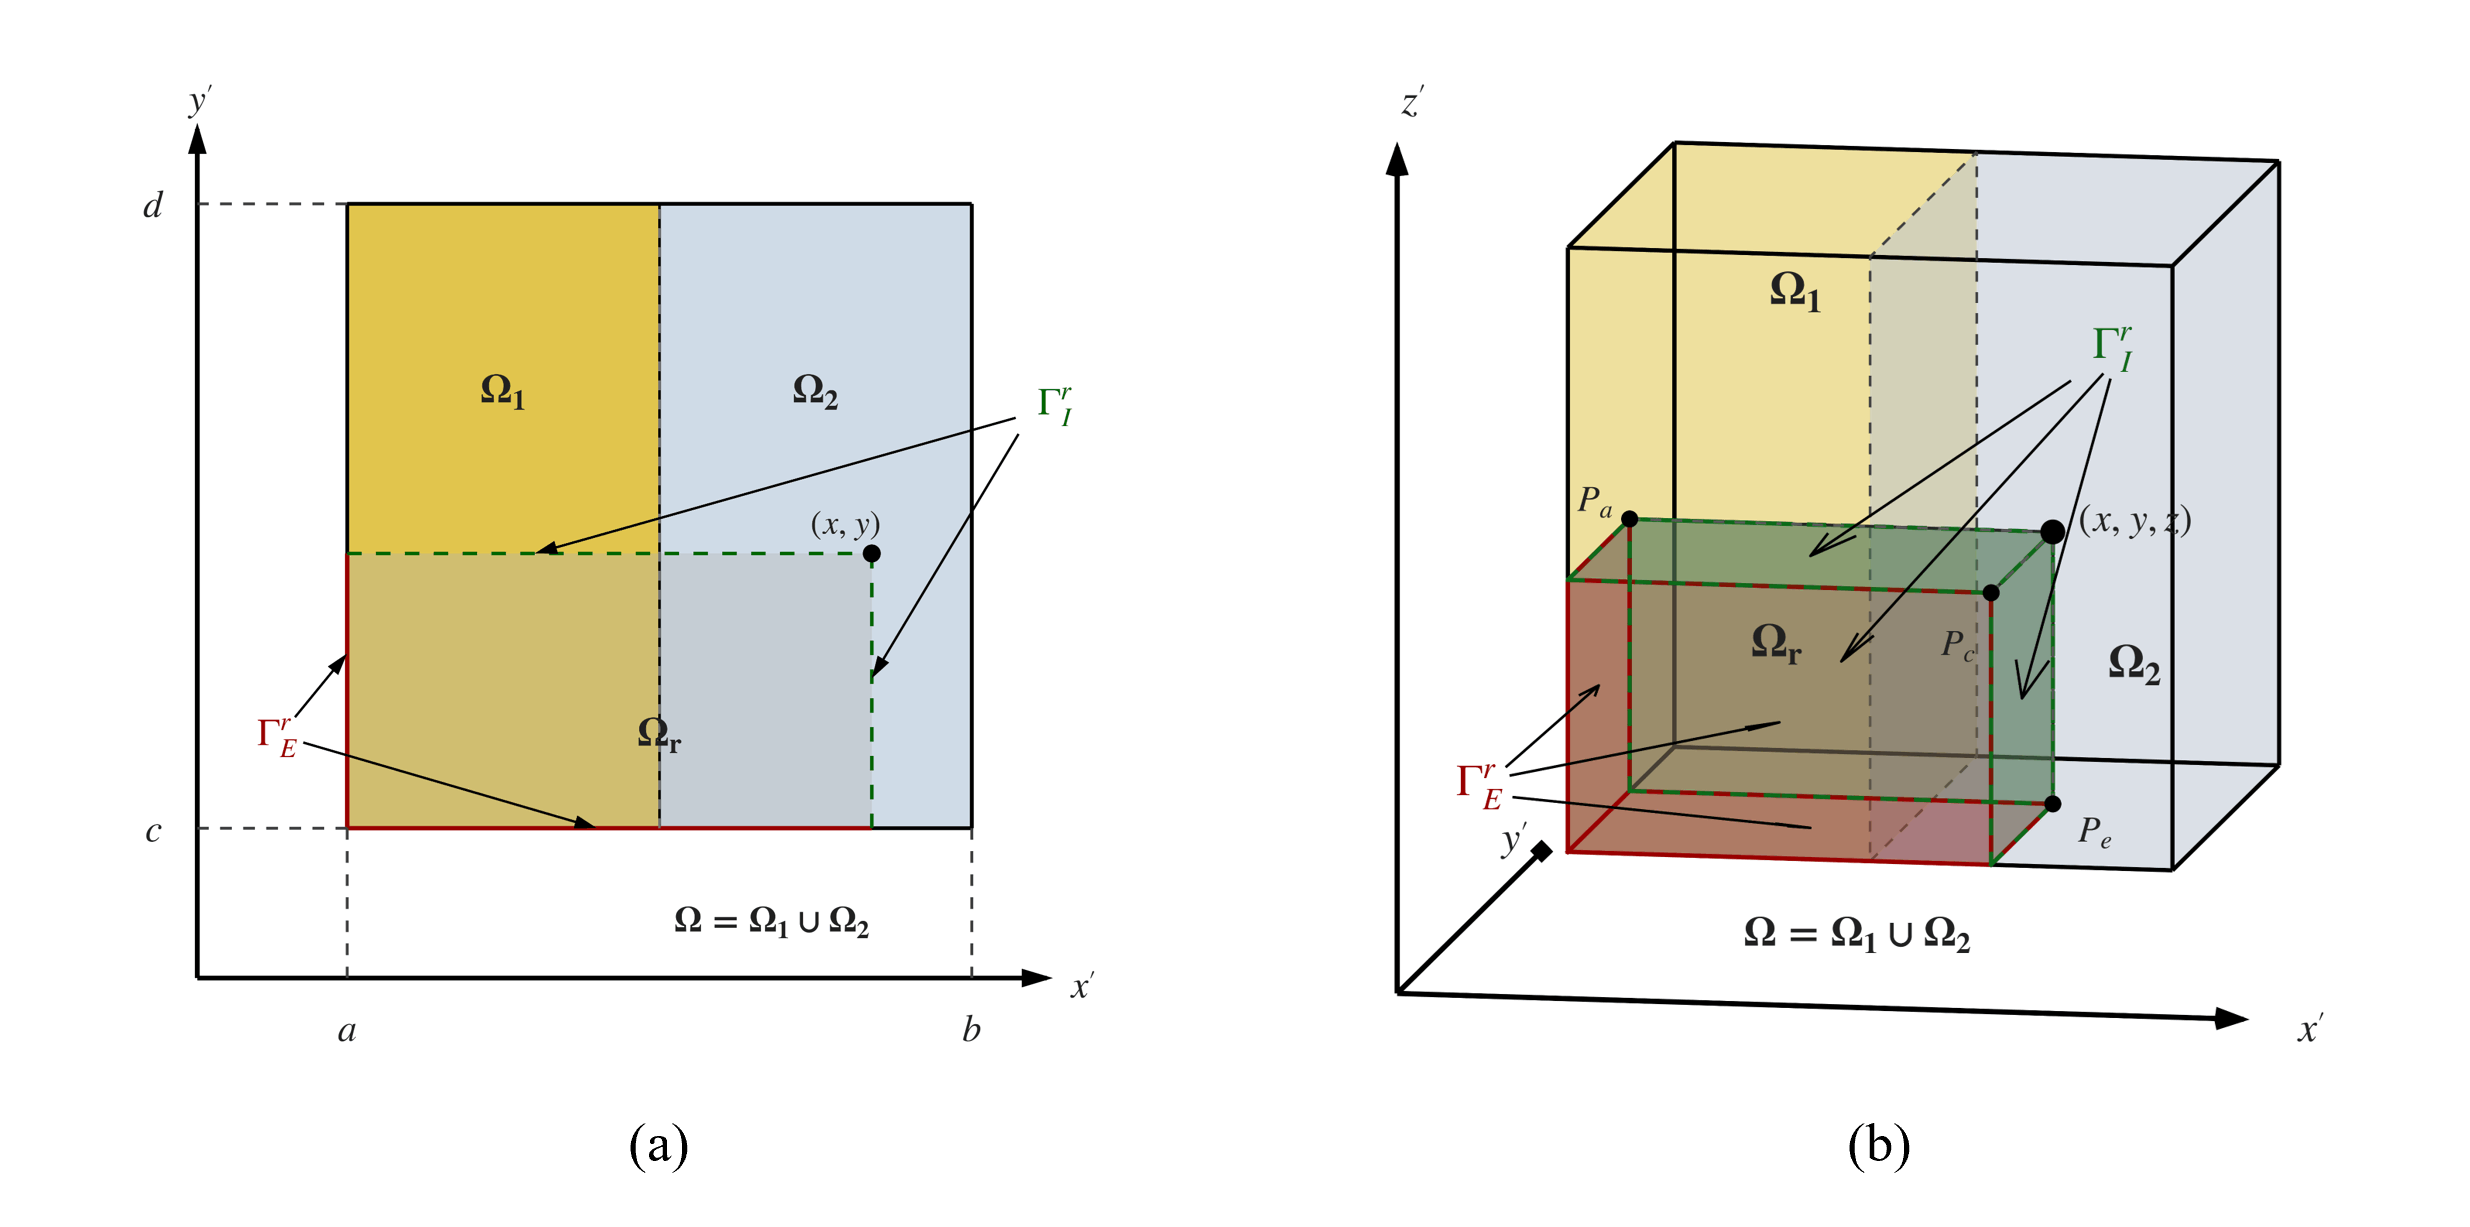
\includegraphics[width=0.7\textwidth]{./fig/figure_00.png}
\caption{Schematic of variable-domain integration regions: (a) two-dimensional rectangular domain; (b) three-dimensional cubic domain.}
\label{fig:two_group_viws_g}
\end{figure}

The weak form is derived below using the first-group equation as an example. By integrating the first equation in \cref{eq:two_group_eigenvalue} over the variable domain $\Omega_{\boldsymbol r}$ and choosing the constant test function $v=1$, for which $\nabla v=0$, we obtain
\begin{equation}
\begin{aligned}
    & \int_{c}^{y} \int_{a}^{x} \left[ -\nabla \cdot \left( D_1(x',y') \nabla \phi_1(x',y') \right) \right] \,dx'dy' \\
    &\quad + \int_{c}^{y} \int_{a}^{x} \left[ \Sigma_{\mathrm a,1}(x',y') + \Sigma_{\mathrm s,1\rightarrow2}(x',y') \right] \phi_1(x',y') \,dx'dy' \\
    &= \frac{1}{k_{\mathrm{eff}}} \int_{c}^{y} \int_{a}^{x} \left[ \nu_1\Sigma_{\mathrm f,1}(x',y')\phi_1(x',y') + \nu_2\Sigma_{\mathrm f,2}(x',y')\phi_2(x',y') \right] \,dx'dy' .
\end{aligned}
\label{eq:two_group_first_variable_integral}
\end{equation}
Since the gradient $\nabla v$ of the constant test function is zero, the above diffusion term can be transformed into a boundary integral form by using the basic weak-solution theory:
\begin{equation}
\int_{c}^{y} \int_{a}^{x} \left[ -\nabla \cdot \left( D_1(x',y') \nabla \phi_1(x',y') \right) \right] dx'dy' = -\oint_{\partial\Omega_{\boldsymbol r}} D_1(x',y') \nabla \phi_1(x',y') \cdot \boldsymbol n d\gamma .
\label{eq:two_group_first_gauss_green}
\end{equation}
For the rectangular subdomain $\Omega_{\boldsymbol r}=[a,x]\times[c,y]$, the outward normal vectors $\boldsymbol n$ on its four boundaries are as follows: $(-1,0)$ at $x'=a$, $(1,0)$ at $x'=x$, $(0,-1)$ at $y'=c$, and $(0,1)$ at $y'=y$. Accordingly, the boundary integral of the diffusion term can be expanded as:
\begin{equation}
\begin{aligned}
     -\oint_{\partial\Omega_{\boldsymbol r}} D_1(x',y') \nabla \phi_1(x',y') \cdot \boldsymbol n d\gamma
    &= \int_{c}^{y} D_1(a,y') \frac{\partial \phi_1}{\partial x'}(a,y') \,dy' - \int_{c}^{y} D_1(x,y') \frac{\partial \phi_1}{\partial x'}(x,y') \,dy' \\
    &\quad + \int_{a}^{x} D_1(x',c) \frac{\partial \phi_1}{\partial y'}(x',c) \,dx' - \int_{a}^{x} D_1(x',y) \frac{\partial \phi_1}{\partial y'}(x',y) \,dx' .
\end{aligned}
\label{eq:two_group_first_boundary_expand}
\end{equation}
Substituting \cref{eq:two_group_first_boundary_expand} into \cref{eq:two_group_first_variable_integral} gives the two-dimensional variable-domain integral weak solution form of the first-group equation. Similarly, by integrating the second-group equation over $\Omega_{\boldsymbol r}$ and rearranging the terms, the corresponding weak-form equation can be obtained.

Therefore, the variable-domain integral weak solution form of the two-dimensional two-group steady-state diffusion eigenvalue problem on the rectangular domain can be written as follows:
\begin{equation}
\left\{
\begin{aligned}
    &
    \int_{c}^{y}
    D_1(a,y')
    \frac{\partial \phi_1}{\partial x'}(a,y')
    \,dy'
    -
    \int_{c}^{y}
    D_1(x,y')
    \frac{\partial \phi_1}{\partial x'}(x,y')
    \,dy'
    \\
    &\quad
    +
    \int_{a}^{x}
    D_1(x',c)
    \frac{\partial \phi_1}{\partial y'}(x',c)
    \,dx'
    -
    \int_{a}^{x}
    D_1(x',y)
    \frac{\partial \phi_1}{\partial y'}(x',y)
    \,dx'
    \\
    &\quad
    +
    \int_{c}^{y}
    \int_{a}^{x}
    \left[
    \Sigma_{\mathrm a,1}(x',y')
    +
    \Sigma_{\mathrm s,1\rightarrow2}(x',y')
    \right]
    \phi_1(x',y')
    \,dx'dy'
    \\
    &=
    \frac{1}{k_{\mathrm{eff}}}
    \int_{c}^{y}
    \int_{a}^{x}
    \left[
    \nu_1\Sigma_{\mathrm f,1}(x',y')\phi_1(x',y')
    +
    \nu_2\Sigma_{\mathrm f,2}(x',y')\phi_2(x',y')
    \right]
    \,dx'dy',
    \\[0.8em]
    &
    \int_{c}^{y}
    D_2(a,y')
    \frac{\partial \phi_2}{\partial x'}(a,y')
    \,dy'
    -
    \int_{c}^{y}
    D_2(x,y')
    \frac{\partial \phi_2}{\partial x'}(x,y')
    \,dy'
    \\
    &\quad
    +
    \int_{a}^{x}
    D_2(x',c)
    \frac{\partial \phi_2}{\partial y'}(x',c)
    \,dx'
    -
    \int_{a}^{x}
    D_2(x',y)
    \frac{\partial \phi_2}{\partial y'}(x',y)
    \,dx'
    \\
    &\quad
    +
    \int_{c}^{y}
    \int_{a}^{x}
    \Sigma_{\mathrm a,2}(x',y')
    \phi_2(x',y')
    \,dx'dy'
    =
    \int_{c}^{y}
    \int_{a}^{x}
    \Sigma_{\mathrm s,1\rightarrow2}(x',y')
    \phi_1(x',y')
    \,dx'dy' .
\end{aligned}
\right.
\label{eq:two_group_variable_weak_form}
\end{equation}

For the three-dimensional problem, let $\boldsymbol r=(x,y,z)$ and let the computational domain be $\Omega=[a,b]\times[c,d]\times[e,f]$. The variable-domain integration region is defined as
\begin{equation}
\Omega_{\boldsymbol r} = [a,x]\times[c,y]\times[e,z].
\label{eq:two_group_variable_domain_3d}
\end{equation}
Its principle is shown in \cref{fig:two_group_viws_g}(b). The derivation in the three-dimensional case is similar to that in the two-dimensional case. The main difference is that the boundary of the variable domain is extended from line segments to surfaces, and the corresponding boundary integrals change from line integrals to surface integrals. In addition, this method can be directly extended to other multigroup diffusion equations.


%====================================================
\subsection{Antiderivative transformation}
\label{subsec:antiderivative_transform}

After constructing the variable-domain integral weak solution form shown in \cref{eq:multigroup_variable_weak_form}, if the variable-domain integral terms are directly treated by traditional numerical integration methods, dense discrete summation will cause a large computational load because deep learning methods involve large-scale iterative optimization \cite{liu2025neutron}. To improve computational efficiency, this paper introduces the antiderivative transformation theory \cite{liu2024repeated}. The aim is to transform variable-domain integral terms with continuous integrands into equivalent local differential constraints, thereby reducing the scale of numerical integral terms that need to be handled.

For the diffusion volume integral term in \cref{eq:multigroup_variable_weak_form}, if the integrand $D_g(\boldsymbol \xi) \nabla \phi_g(\boldsymbol \xi) \cdot \nabla v(\boldsymbol \xi)$ is continuous in the integration domain, then according to the Newton--Leibniz formula \cite{courant1999introduction} and related theory \cite{liu2024repeated}, an antiderivative $F_{g,0}(\boldsymbol r)$ can be defined to satisfy the following differential-integral relation:
\begin{equation}
    \left\{
    \begin{aligned}
        F_{g,0}(\boldsymbol r) &= \int_{\Omega_{\boldsymbol r}} D_g(\boldsymbol \xi) \nabla \phi_g(\boldsymbol \xi) \cdot \nabla v(\boldsymbol \xi) \,d\boldsymbol \xi , \\
        \frac{\partial^d F_{g,0}}{\partial r_1\partial r_2\cdots\partial r_d} &= D_g(\boldsymbol r) \nabla \phi_g(\boldsymbol r) \cdot \nabla v(\boldsymbol r) .
    \end{aligned}
    \right.
    \label{eq:Fg0_integral}
\end{equation}

Since the family of antiderivatives differs by a function term $C(\boldsymbol{r})$ related to $\boldsymbol{r}$ \cite{courant1999introduction}, a specific condition must be introduced to ensure uniqueness, denoted as $F_{g,0}({\boldsymbol{r}}_{a}) = {g}_{a}$. The construction and detailed discussion of such conditions can be found in Refs. \cite{liu2024repeated, liu2026variabledomain, liu2026supplementary}.

Similarly, for the boundary integral terms in \cref{eq:multigroup_variable_weak_form}, if the integrand $\left[ -D_g(\boldsymbol \xi) \nabla \phi_g(\boldsymbol \xi) \cdot \boldsymbol n \right] v(\boldsymbol \xi)$ satisfies the continuity requirement, it can be decomposed along the coordinate directions. Under the condition $F_{g,\ell}(\boldsymbol r_b) = {g}_{\ell}$, the antiderivative $F_{g,\ell}(\boldsymbol r)$ corresponding to the $\ell$-th coordinate direction can be determined. Through the above transformation, the original variable-domain integral weak solution form \cref{eq:multigroup_variable_weak_form} can finally be transformed into the following antiderivative-transformed weak solution form:
\begin{equation}
    \begin{aligned}
    & F_{g,0}(\boldsymbol r) - \sum_{\ell=1}^{d}F_{g,\ell}(\boldsymbol r) + \int_{\Omega_{\boldsymbol r}} \Sigma_{t,g}(\boldsymbol \xi) \phi_g(\boldsymbol \xi) v(\boldsymbol \xi) \,d\boldsymbol \xi \\
    \quad & =
    \int_{\Omega_{\boldsymbol r}}
    \left[
    \sum_{g'=1}^{G}
    \Sigma_{\mathrm{s},g'\to g}(\boldsymbol \xi)
    \phi_{g'}(\boldsymbol \xi)
    +
    \frac{\chi_g}{k_{\mathrm{eff}}}
    \sum_{g'=1}^{G}
    \left(\nu\Sigma_{\mathrm{f}}\right)_{g'}(\boldsymbol \xi)
    \phi_{g'}(\boldsymbol \xi)
    \right]
    v(\boldsymbol \xi)\,d\boldsymbol \xi ,
    \qquad g=1,2,\ldots,G .
    \end{aligned}
    \label{eq:variable_order_mg_main}
\end{equation}

%====================================================
\subsection{Deep learning solution of the antiderivative-transformed weak solution form}
\label{sec:nn_loss}

After obtaining the antiderivative-transformed form shown in \cref{eq:variable_order_mg_main}, it can be solved based on the classical PINN architecture \cite{raissi2019physicsinformed} or improved deep learning frameworks for differential equations \cite{sengupta2020review, wang2024multistage}. In this paper, neural networks are used to approximate the neutron fluxes of all energy groups and the corresponding antiderivatives. For the $g$-th energy group, the neutron flux is written as
\begin{equation}
\phi_{g,\theta}(\boldsymbol r)
=
\mathcal{N}_{\phi_g}(\boldsymbol r;\theta_g),
\qquad g=1,2,\ldots,G ,
\label{eq:nn_phi_g}
\end{equation}
where $\mathcal{N}_{\phi_g}$ is the neutron flux network of the $g$-th group, and $\theta_g$ denotes its network parameters.

Similarly, the antiderivative terms can be written as
\begin{equation}
F_{g,m,\eta}(\boldsymbol r)
=
\mathcal{N}_{F_{g,m}}(\boldsymbol r;\eta_{g,m}),
\qquad
m=0,1,\ldots,d .
\label{eq:nn_F_g}
\end{equation}
Here, $F_{g,0,\eta}$ corresponds to the antiderivative of the diffusion volume integral term, and $F_{g,\ell,\eta}$ corresponds to the boundary flux antiderivative in the $\ell$-th coordinate direction, with $\ell=1,2,\ldots,d$. In practical implementation, independent networks can be built for different antiderivatives, or a multi-output neural network can be used to represent several antiderivative components together.

Based on the above approximations, the total loss function consists of the equation residual, the antiderivative definition constraint, the antiderivative determining conditions, and the boundary conditions:

\begin{equation}
    \mathcal{L}
    =
    w_{\mathrm r}\mathcal{L}_{\mathrm r}
    +
    w_{\mathrm{def}}\mathcal{L}_{\mathrm{def}}
    +
    w_F\mathcal{L}_{F}
    +
    w_{\mathrm b}\mathcal{L}_{\mathrm b},
    \label{eq:total_loss_viws}
\end{equation}
where $\mathcal{L}_{\mathrm r}$ is used to constrain the equation residual shown in \cref{eq:variable_order_mg_main}; $\mathcal{L}_{\mathrm{def}}$ is used to constrain the differential relation between the antiderivatives and their corresponding integrands; $\mathcal{L}_{F}$ is used to impose the determining conditions of the antiderivatives; and $\mathcal{L}_{\mathrm b}$ is used to satisfy the boundary conditions shown in \cref{eq:mg_bc}. $w_{\mathrm r}$, $w_{\mathrm{def}}$, $w_F$, and $w_{\mathrm b}$ are the corresponding loss weights. 

It should be noted that the diffusion volume integral term and part of the boundary flux terms in \cref{eq:variable_order_mg_main} that satisfy the continuity requirements are constrained by the antiderivative networks and their automatic differentiation. In contrast, the absorption, scattering, and fission source terms usually contain material-dependent macroscopic cross sections and may have jumps at interfaces in multi-material problems, so they are calculated by numerical integration. In this way, the number of terms that need direct numerical integration is reduced, while avoiding the forced construction of global antiderivatives for discontinuous terms.
During training, all neural-network parameters are optimized to minimize the total loss function in \cref{eq:total_loss_viws}. When the loss value reaches the preset accuracy requirement or satisfies the stopping criterion, $\mathcal{N}_{\phi_g}(\boldsymbol r;\theta_g)$ is used as the numerical approximation of the group-$g$ neutron flux $\phi_g(\boldsymbol r)$. Related implementation details can be found in Refs. \cite{liu2025neutron, liu2024repeated}.

\section{Numerical experiments}
\label{sec:numerical_experiments}

This section presents a series of numerical examples to evaluate the ability of the VIWS method to solve neutron diffusion equations with discontinuous coefficients. The reference solutions are obtained by the high-accuracy FEM, and the comparison method is the standard PINN~\cite{raissi2019physicsinformed}.
Unless otherwise stated, the examples use the same basic training protocol. The weights of the loss terms, $w_{\mathrm r}$, $w_{\mathrm{def}}$, $w_F$, and $w_{\mathrm b}$, are selected according to the physical meanings of the constraints and empirical numerical tests; in general, the boundary-condition weight is set larger than the interior residual weights to improve boundary satisfaction. A two-stage training strategy combining Adam and L-BFGS is used. In the Adam stage, the learning rate is $10^{-3}$ and the number of iterations is $2,000$. Then, L-BFGS is used for further optimization until the loss function satisfies the convergence criterion. The default network is an 8-layer fully connected neural network, with 32 neurons in each layer and Tanh as the activation function.

The prediction accuracy is measured by the relative $L_2$ error:
\begin{equation}
\label{eq:l2_error}
\epsilon_{L_2}
=
\frac{\|\hat{\phi}-\phi_{\mathrm{ref}}\|_2}
{\|\phi_{\mathrm{ref}}\|_2}
=
\sqrt{
\frac{
\sum_{i=1}^{N}
\left(
\hat{\phi}(\boldsymbol r_i)-\phi_{\mathrm{ref}}(\boldsymbol r_i)
\right)^2
}{
\sum_{i=1}^{N}
\phi_{\mathrm{ref}}^2(\boldsymbol r_i)
}
}.
\end{equation}
where $\hat{\phi}$ is the neutron flux predicted by the neural network, $\phi_{\mathrm{ref}}$ is the FEM reference flux, and $N$ is the number of test points. For eigenvalue problems, the deviation of the effective multiplication factor is expressed in pcm, namely
$\Delta k_{\mathrm{pcm}}=|k_{\mathrm{NN}}-k_{\mathrm{ref}}|\times 10^5$.

%=============================================================
\subsection{2D regular hexagonal single-group fixed-source problem}
\label{subsec:case1}

This example considers a single-group fixed-source problem in a two-dimensional regular hexagonal domain. It is used to test the performance of VIWS for problems with complex outer boundaries. The single-group fixed-source equation corresponding to \cref{eq:multigroup_fixed_source} is
\begin{equation}
-\nabla\cdot \left( D(\boldsymbol r)\nabla\phi(\boldsymbol r) \right) + \Sigma_{\mathrm{t}}(\boldsymbol r)\phi(\boldsymbol r) = \nu\Sigma_{\mathrm{f}}(\boldsymbol r)\phi(\boldsymbol r) + S(\boldsymbol r), \quad \boldsymbol r\in\Omega
\label{eq:single_group_diffusion}
\end{equation}
where $\boldsymbol r=(x,y)$, and $\phi$ is the single-group neutron flux. A homogeneous Dirichlet condition is imposed on the outer boundary:
$\phi(\boldsymbol r)=0,\ \boldsymbol r\in\partial\Omega.$

The computational domain $\Omega$ is a regular hexagon with a circumradius of $R=1.0\ \mathrm{cm}$. It is divided into three subdomains, $\Omega_1$, $\Omega_2$, and $\Omega_3$, by two concentric circular interfaces. \cref{fig:case1_geometry_reference_testfunction}(a) shows the geometry and material regions, and \cref{fig:case1_geometry_reference_testfunction}(b) shows the FEM reference flux. The material parameters are listed in \cref{tab:case1_material_parameters}.


\begin{table}[H]
    \centering
    \caption{Material parameters for the 2D regular hexagonal single-group fixed-source problem}
    \label{tab:case1_material_parameters}
    \small
    \begin{tabularx}{0.95\textwidth}{@{\extracolsep{\fill}}cccccc}
        \toprule
        Subdomain         & Radial range               & $D$\,(cm) & $\Sigma_{\mathrm{t}}$\,(cm$^{-1}$) & $\nu\Sigma_{\mathrm{f}}$\,(cm$^{-1}$) & $S$ (cm$^{-3}\cdot$s$^{-1}$) \\
        \midrule
        $\Omega_1$ & $r \le 0.5$        & 1.00      & 0.220                              & 0.120                                 & 10                       \\
        $\Omega_2$ & $0.5 < r \le 0.65$ & 0.25      & 0.060                              & 0.000                                 & 0                        \\
        $\Omega_3$ & $r > 0.65$         & 4.00      & 0.020                              & 0.000                                 & 0                        \\
        \bottomrule
    \end{tabularx}
\end{table}

\begin{figure}[H]
\centering
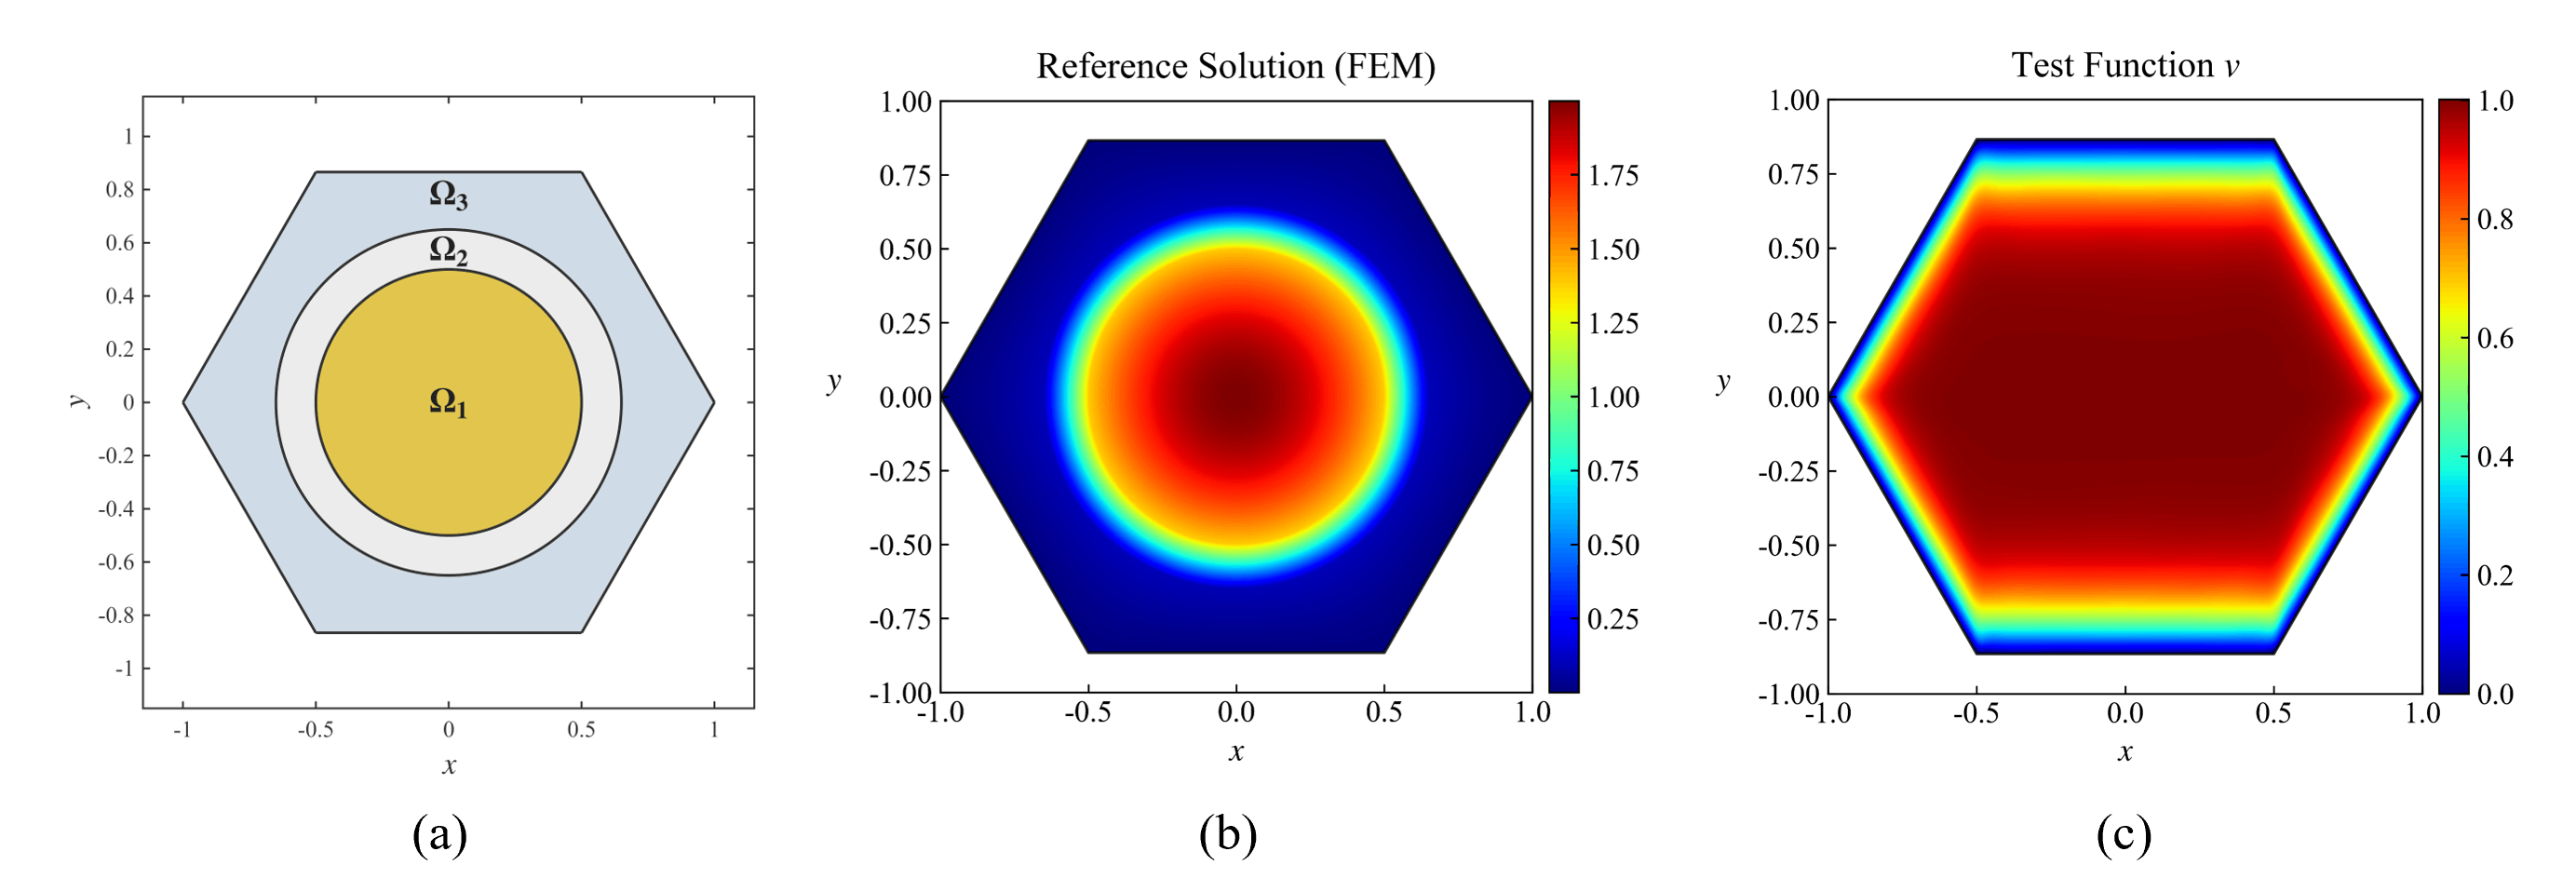
\includegraphics[width=0.85\textwidth]{fig/figure_01.png}
\caption{Computational setup of the 2D regular hexagonal single-group fixed-source problem. (a) Geometry and material regions; (b) FEM reference flux; (c) neural-network test function $v$.}
\label{fig:case1_geometry_reference_testfunction}
\end{figure}
VIWS uses four independent neural networks to represent the neutron flux $\phi(x,y)$ and the antiderivatives $\{F_k\}_{k=0}^{2}$, respectively. The total number of interior and boundary sampling points is $10,000$. For the regular hexagonal boundary, this paper uses a bell-shaped neural-network test function that is zero on $\partial\Omega$. Its spatial distribution is shown in \cref{fig:case1_geometry_reference_testfunction}(c).


\cref{fig:case1_flux_error_comparison} compares the flux predictions and absolute errors of the standard PINN and VIWS. The relative $L_2$ error of the standard PINN is $4.04\times10^{-1}$, and the error is mainly concentrated near the source region $\Omega_1$. The relative $L_2$ error of VIWS is reduced to $1.25\times10^{-2}$. \cref{fig:case1_antiderivative_fields} shows the antiderivative fields $F_0$, $F_1$, and $F_2$ learned by VIWS. The results indicate that VIWS is applicable to problems with complex outer boundaries and achieves substantially higher accuracy than the standard PINN.

\begin{figure}[H]
\centering
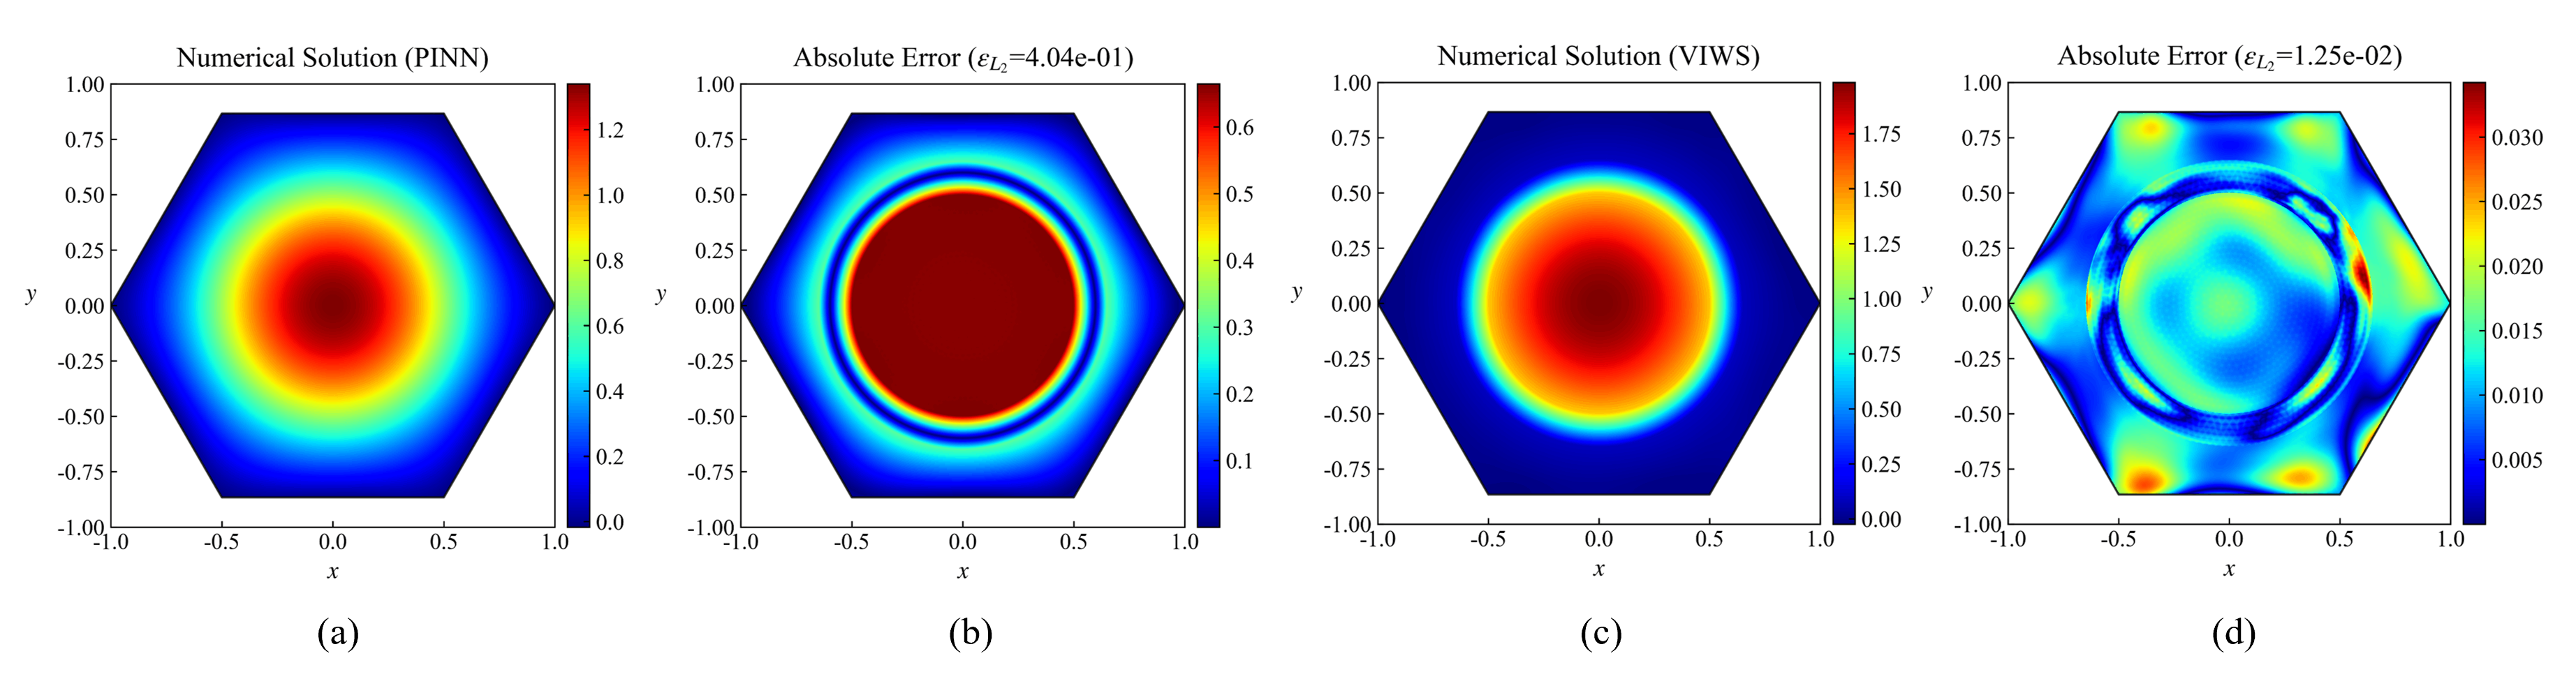
\includegraphics[width=1\textwidth]{fig/figure_02.png}
\caption{Comparison of flux prediction and error for the 2D regular hexagonal single-group fixed-source problem. (a) PINN-predicted flux; (b) PINN absolute error; (c) VIWS-predicted flux; (d) VIWS absolute error.}
\label{fig:case1_flux_error_comparison}
\end{figure}

\begin{figure}[H]
\centering
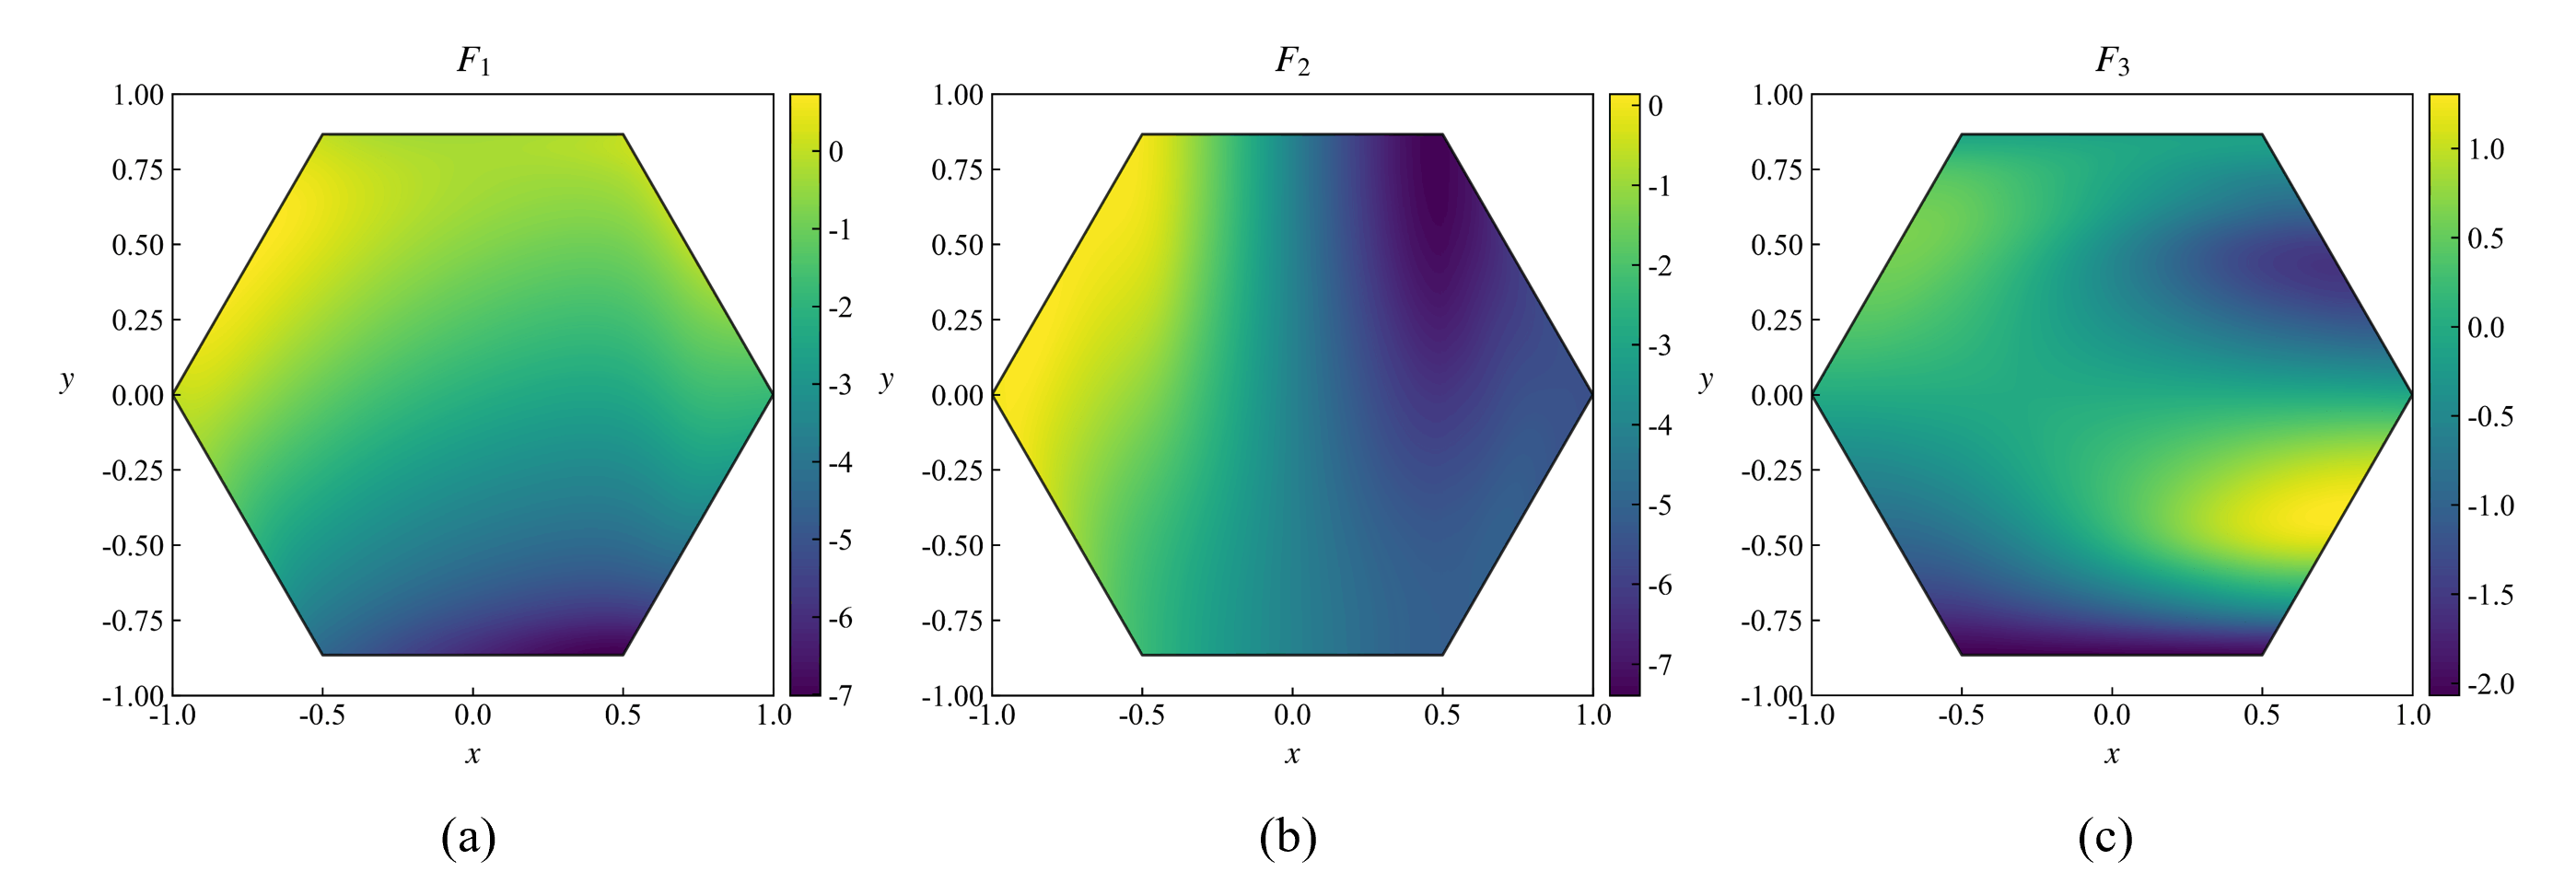
\includegraphics[width=0.75\textwidth]{fig/figure_03.png}
\caption{Antiderivative fields for the 2D regular hexagonal single-group fixed-source problem. (a) $F_0$; (b) $F_1$; (c) $F_2$.}
\label{fig:case1_antiderivative_fields}
\end{figure}


%=============================================================
\subsection{3D eight-region single-group fixed-source problem}
\label{subsec:case2}

This example tests the performance of VIWS for a three-dimensional multi-interface problem in heterogeneous media. The governing equation is still \cref{eq:single_group_diffusion}, where $\boldsymbol r=(x,y,z)$, and homogeneous Dirichlet conditions are imposed on the outer boundary.
The computational domain is $\Omega=[-1,1]^3$. 

The three coordinate planes divide the cube into eight subdomains, $\Omega_1,\ldots,\Omega_8$. \cref{fig:case2_geometry_reference}(a) shows the geometry and material regions, and \cref{fig:case2_geometry_reference}(b) shows the FEM reference flux. The material parameters are listed in \cref{tab:case2_material_parameters}.

\begin{table}[H]
    \centering
    \caption{Material parameters for the 3D eight-region single-group fixed-source problem}
    \label{tab:case2_material_parameters}
    \small
    \begin{tabularx}{0.95\textwidth}{@{\extracolsep{\fill}}ccccc}
        \toprule
        Subdomain                                       & $D$ (cm) & $\Sigma_{\mathrm{t}}$ (cm$^{-1}$) & $\nu\Sigma_{\mathrm{f}}$ (cm$^{-1}$) & $S$ (cm$^{-3}\cdot$s$^{-1}$) \\
        \midrule
        $\Omega_1, \Omega_3, \Omega_6, \Omega_8$ & 1.00     & 0.220                             & 0.120                                & 10.0                    \\
        $\Omega_2, \Omega_4, \Omega_5, \Omega_7$ & 4.00     & 0.020                             & 0.000                                & 0.0                     \\
        \bottomrule
    \end{tabularx}
\end{table}

\begin{figure}[H]
    \centering
    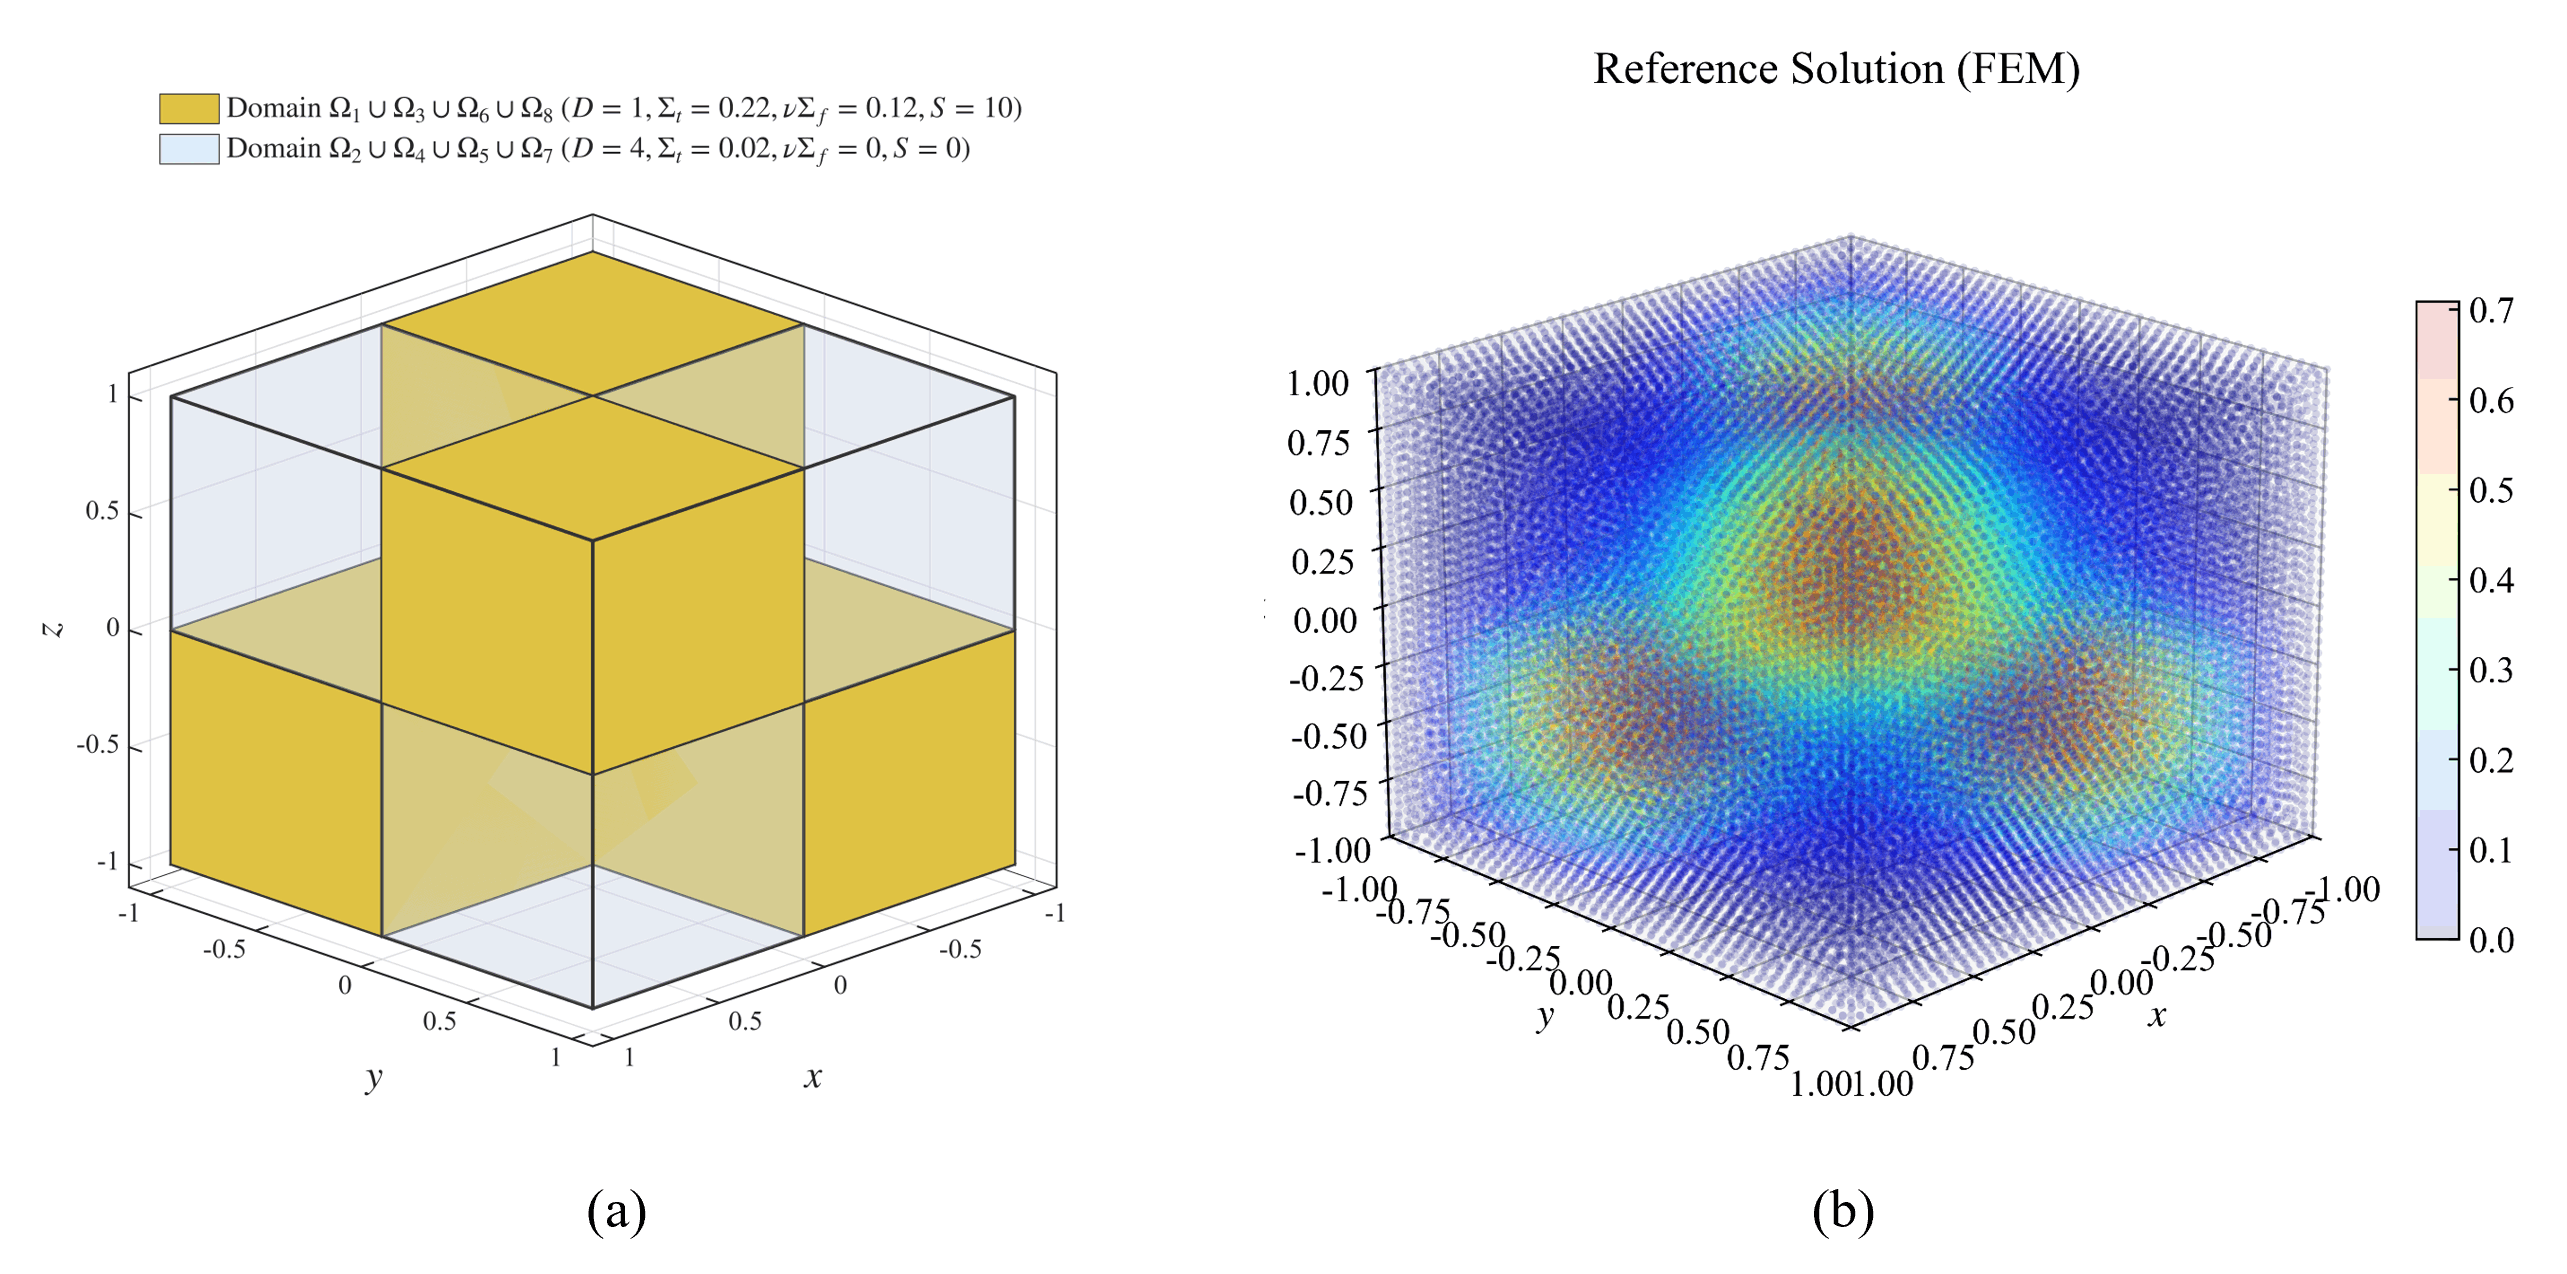
\includegraphics[width=0.55\textwidth]{fig/figure_04.png}
    \caption{Computational setup of the 3D eight-region single-group fixed-source problem. (a) Geometry and material regions; (b) FEM reference flux.}
    \label{fig:case2_geometry_reference}
\end{figure}
In this example, the test function
$v=(x+1)(y+1)(z+1)$
is chosen, which is zero on part of the boundary. Five independent neural networks are used to represent $\phi(x,y,z)$ and $\{F_k\}_{k=0}^{3}$, and the number of sampling points is $216,000$.

\cref{fig:case2_flux_error_comparison} shows the flux predictions and error distributions of the standard PINN and VIWS. The standard PINN produces obvious errors at internal interfaces and interface intersection regions, and its relative $L_2$ error is $3.20\times10^{-1}$. The relative $L_2$ error of VIWS is $2.60\times10^{-2}$. \cref{fig:case2_antiderivative_fields} shows the corresponding antiderivatives $F_0$, $F_1$, $F_2$, and $F_3$ learned by VIWS. 
\begin{figure}[H]
    \centering
    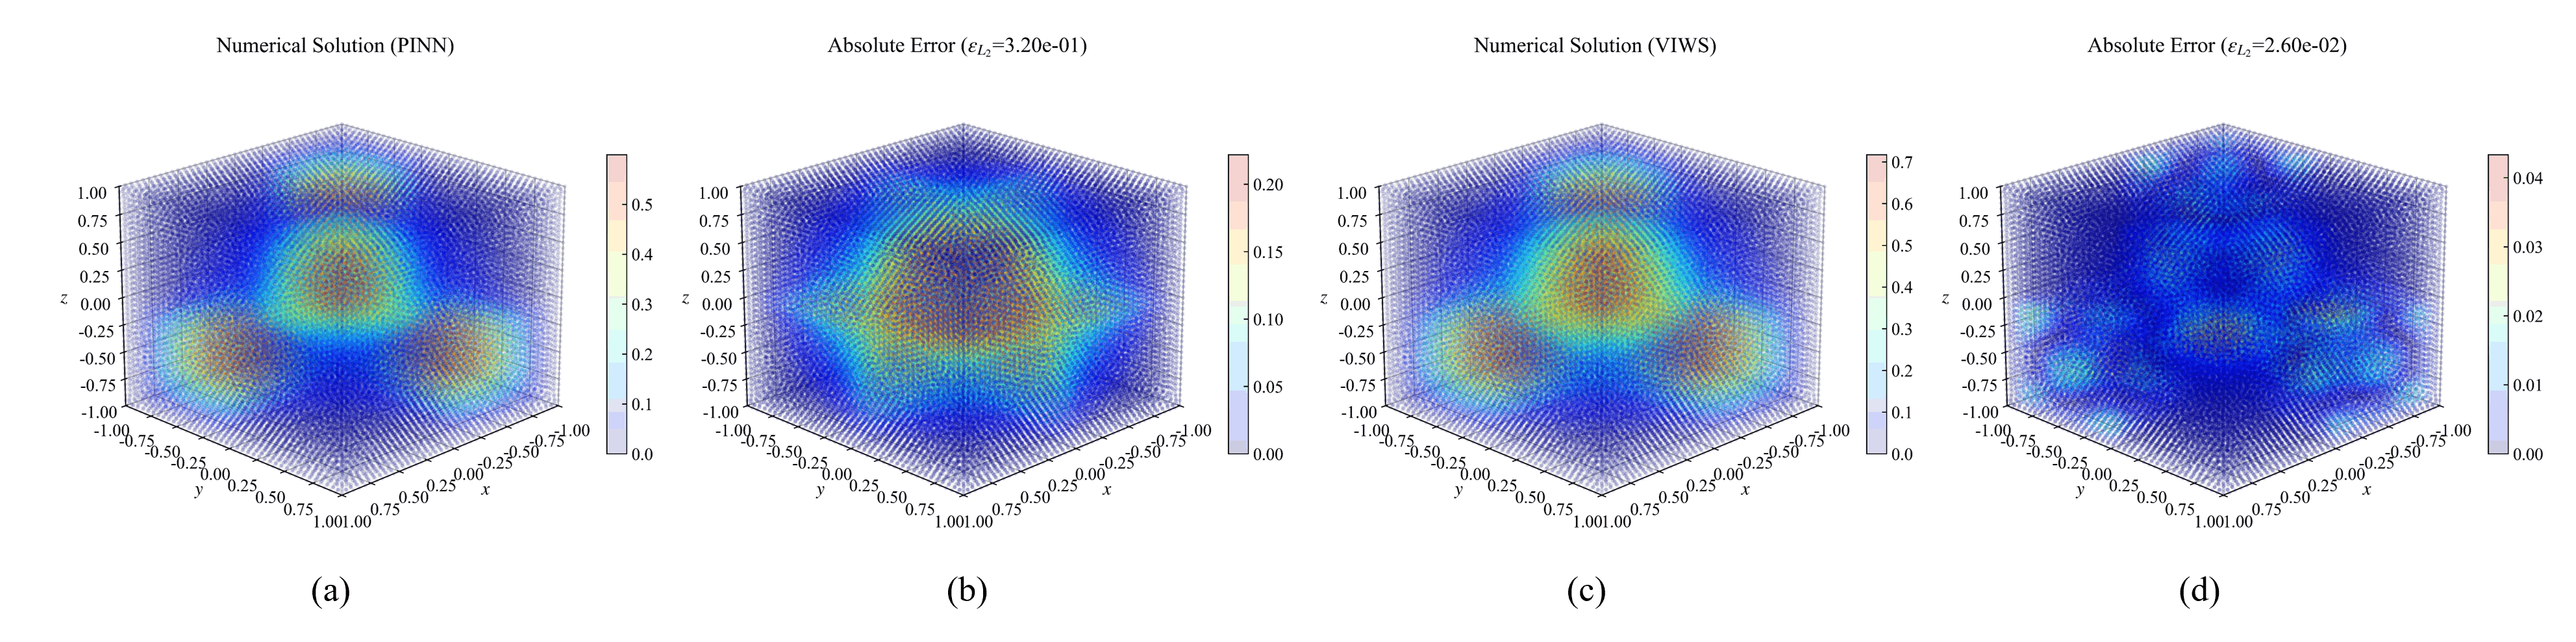
\includegraphics[width=1\textwidth]{fig/figure_05.png}
    \caption{Comparison of flux prediction and error for the 3D eight-region single-group fixed-source problem. (a) PINN-predicted flux; (b) PINN absolute error; (c) VIWS-predicted flux; (d) VIWS absolute error.}
    \label{fig:case2_flux_error_comparison}
\end{figure}

\begin{figure}[H]
    \centering
    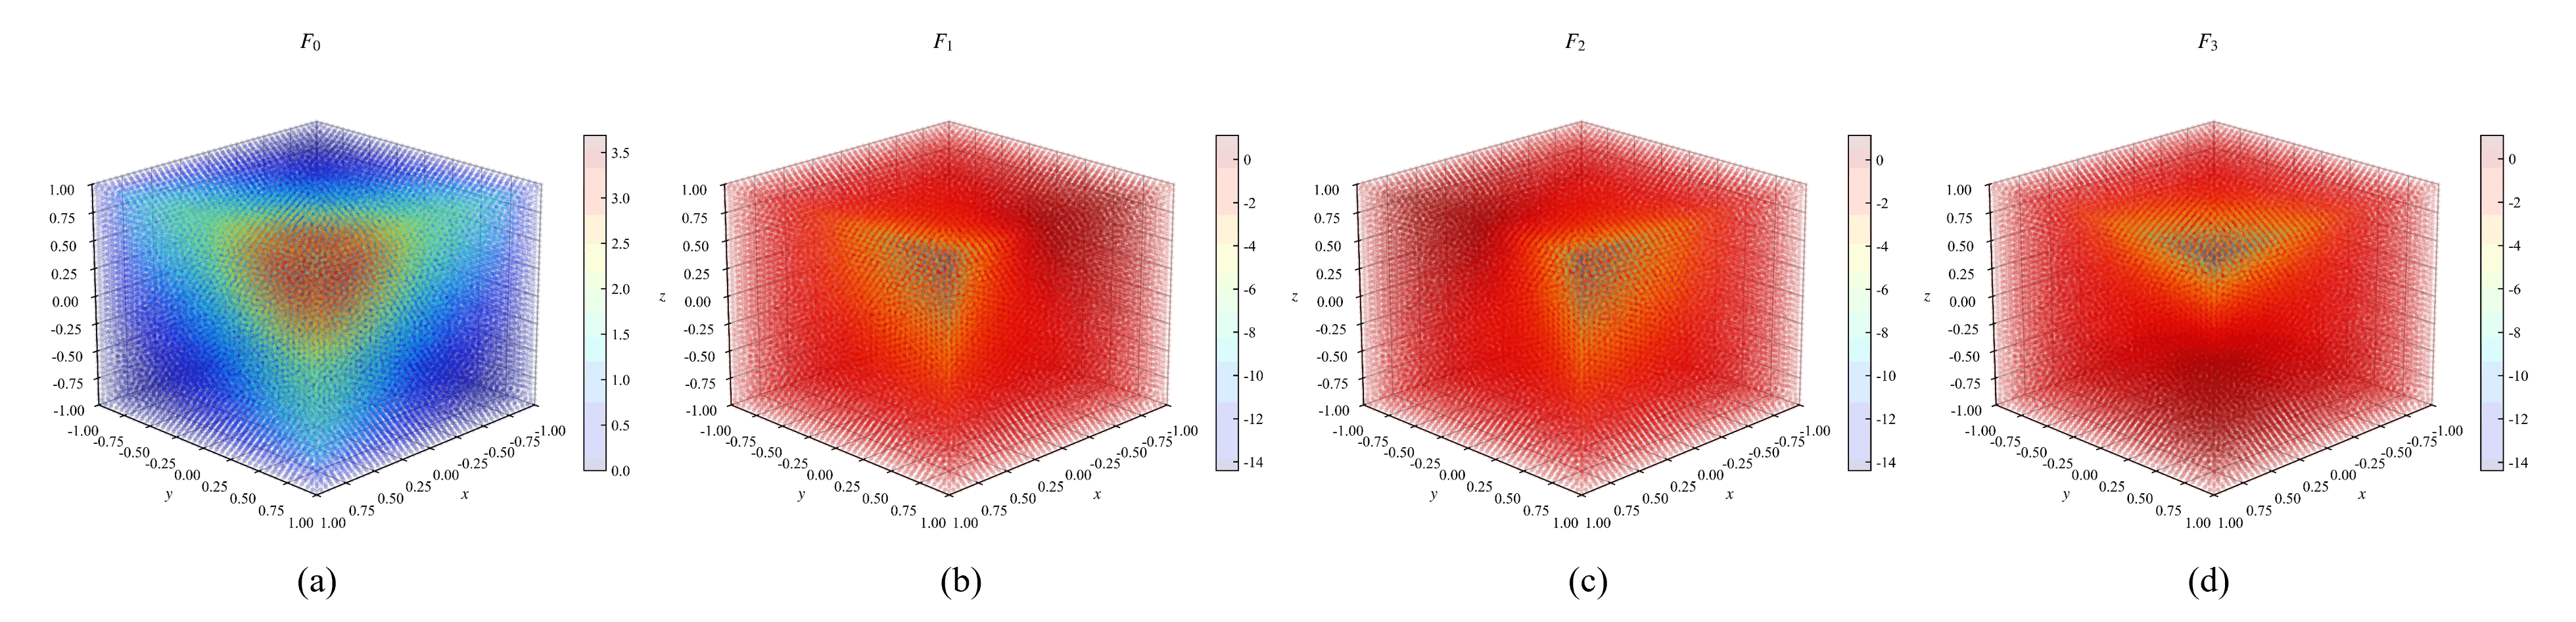
\includegraphics[width=1\textwidth]{fig/figure_06.png}
    \caption{Antiderivative fields for the 3D eight-region single-group fixed-source problem. (a) $F_0$; (b) $F_1$; (c) $F_2$; (d) $F_3$.}
    \label{fig:case2_antiderivative_fields}
\end{figure}

The results show that the proposed method can effectively handle the discontinuity of flux gradients caused by interfaces in high-dimensional heterogeneous media. The proposed method maintains a clear accuracy advantage over the standard PINN. Since this type of diffusion calculation based on regular 3D blocks is common in the engineering design and analysis of large reactor cores \cite{liu2024deep}, this example also verifies the applicability of the proposed method to three-dimensional multi-interface problems from the perspective of engineering application.

%=============================================================
\subsection{3D single-group fixed-source problem with a cylindrical rod bundle array} \label{subsec:case3}

This example further verifies the applicability of the VIWS method for problems with multiple curved interfaces and mixed boundary conditions by considering a three-dimensional array of axially aligned cylindrical rods. The governing equation is \cref{eq:single_group_diffusion}, where the spatial position is denoted by $\boldsymbol r=(x,y,z)$.

The computational domain is set as the cubic region $\Omega=[-1,1]^3$. To simulate typical physical boundaries of a reactor core, homogeneous Dirichlet conditions ($\phi=0$) are imposed on the side boundaries, while zero-normal-gradient Neumann conditions are imposed on the upper and lower surfaces ($z=\pm1$), that is, $\nabla\phi \cdot \boldsymbol{n} = 0$. Inside the computational domain, nine fuel cylinders penetrating along the $z$-axis are uniformly arranged. The geometric layout and material regions are shown in \cref{fig:case3_geometry_reference}(a), and the material parameters are listed in \cref{tab:case3_material_parameters}. In addition, the reference flux field generated by the FEM is shown in \cref{fig:case3_geometry_reference}(b).

\begin{table}[H]
    \centering
    \small
    \caption{Material parameters for the 3D single-group fixed-source problem with a cylindrical rod bundle array}
    \label{tab:case3_material_parameters}
    \begin{tabularx}{0.95\textwidth}{@{\extracolsep{\fill}}ccccc}
        \toprule
        Subdomain                                       & $D$ (cm) & $\Sigma_{\mathrm{t}}$ (cm$^{-1}$) & $\nu\Sigma_{\mathrm{f}}$ (cm$^{-1}$) & $S$ (cm$^{-3}\cdot$s$^{-1}$) \\ 
        \midrule
        $\Omega_{1}$ & 1.00     & 0.220                             & 0.120                                & 10.0                    \\
        $\Omega_{2}$ & 2.00     & 0.010                             & 0.000                                & 0                       \\
        \bottomrule
    \end{tabularx}
\end{table}

\begin{figure}[H]
    \centering
    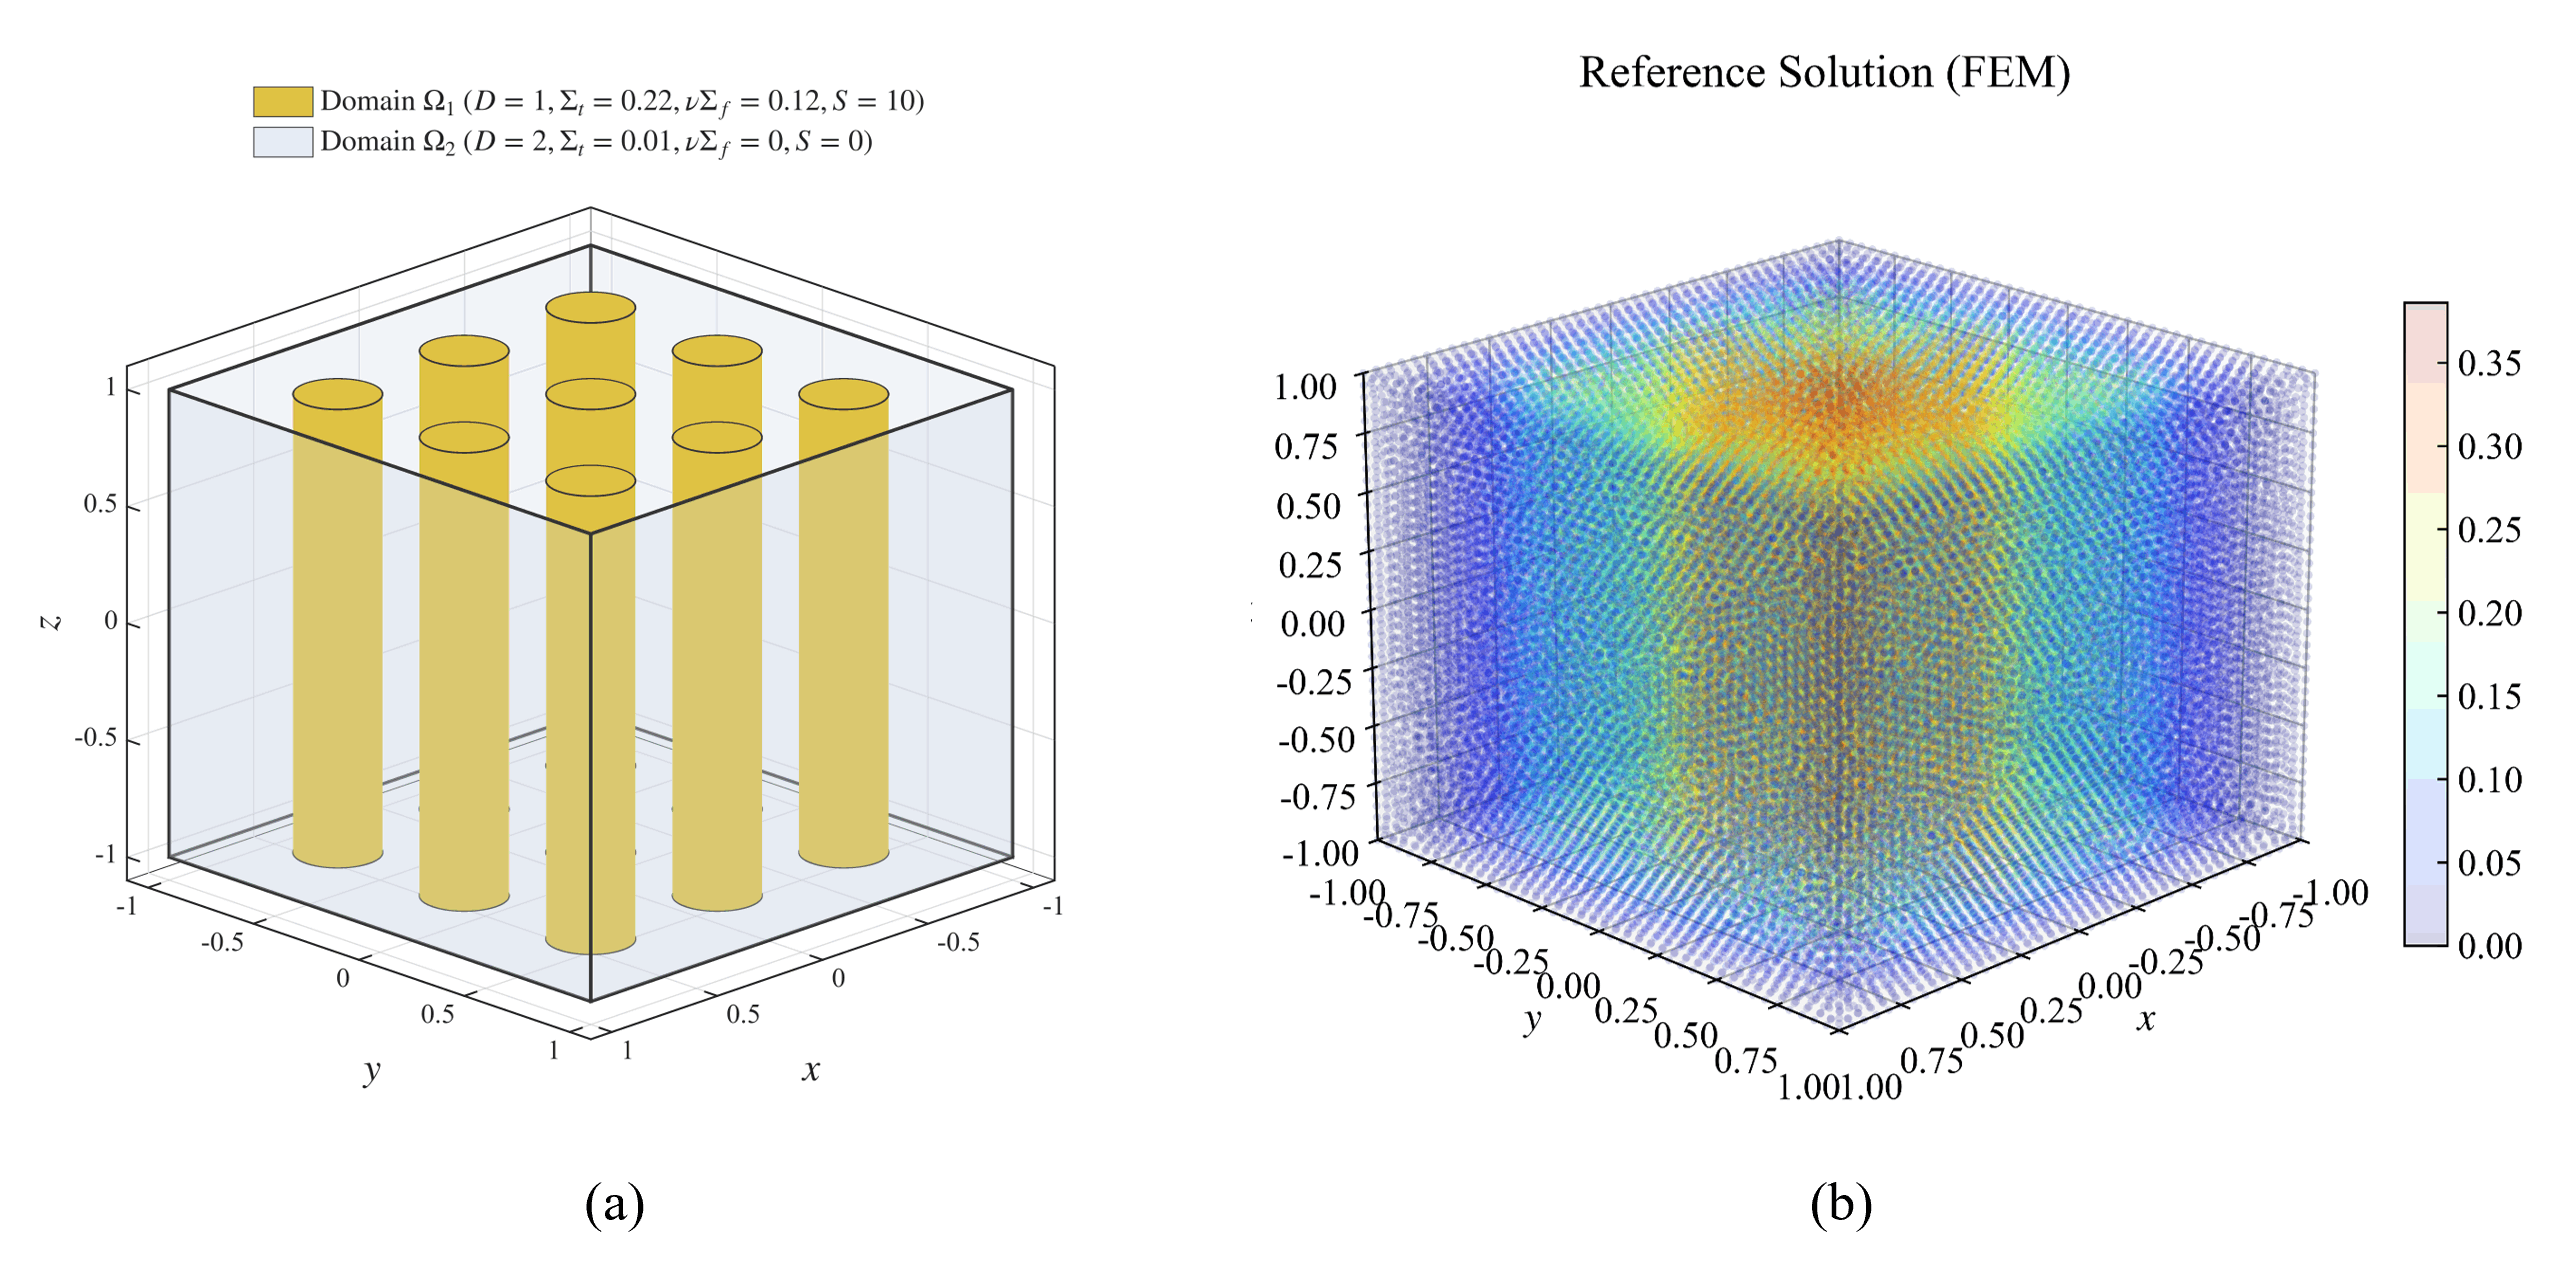
\includegraphics[width=0.55\textwidth]{fig/figure_07.png}
    \caption{Computational setup of the 3D single-group fixed-source problem with a cylindrical rod bundle array. (a) Geometry and material regions; (b) FEM reference flux.}
    \label{fig:case3_geometry_reference}
\end{figure}

In this example, the test function is taken as $v=1$, and the other hyperparameters are the same as those in \cref{subsec:case2}. \cref{fig:case3_flux_error_comparison} shows the flux predictions and error distributions of the standard PINN and VIWS. The relative $L_2$ error of the standard PINN is $3.55\times10^{-1}$, while that of VIWS is $6.26\times10^{-2}$. \cref{fig:case3_antiderivative_fields} shows the corresponding antiderivatives $F_0$, $F_1$, $F_2$, and $F_3$.

\begin{figure}[H]
    \centering
    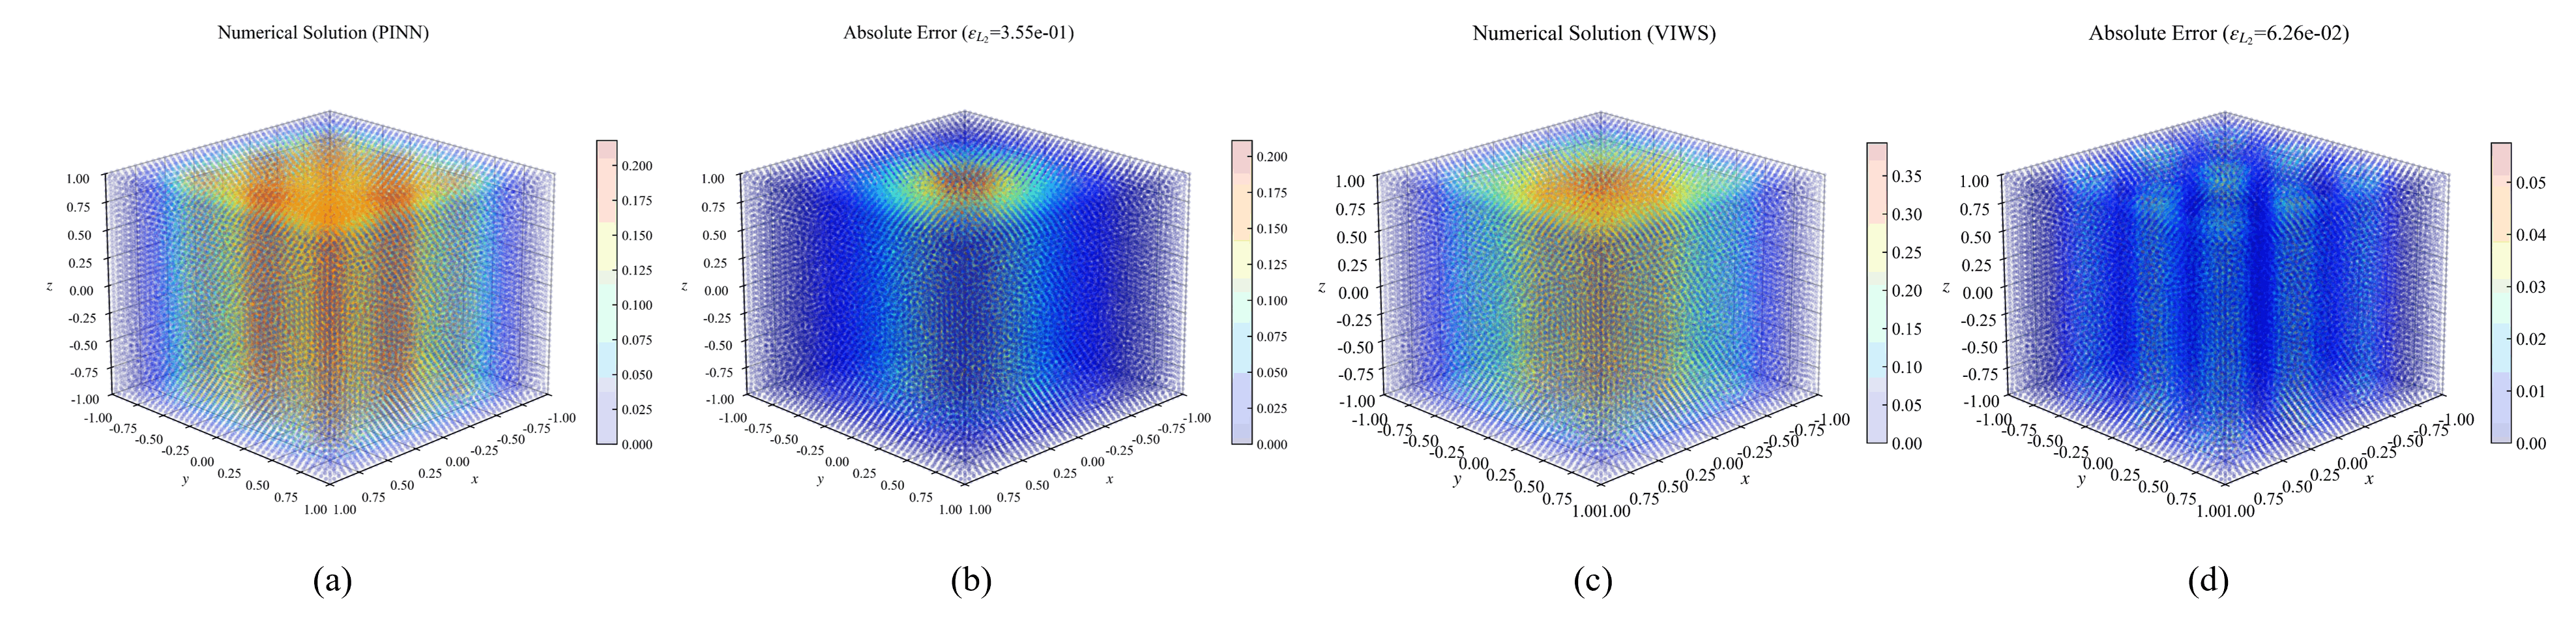
\includegraphics[width=1\textwidth]{fig/figure_08.png}
    \caption{Comparison of flux prediction and error for the 3D single-group fixed-source problem with a cylindrical rod bundle array. (a) PINN-predicted flux; (b) PINN absolute error; (c) VIWS-predicted flux; (d) VIWS absolute error.}
    \label{fig:case3_flux_error_comparison}
\end{figure}

\begin{figure}[H]
    \centering
    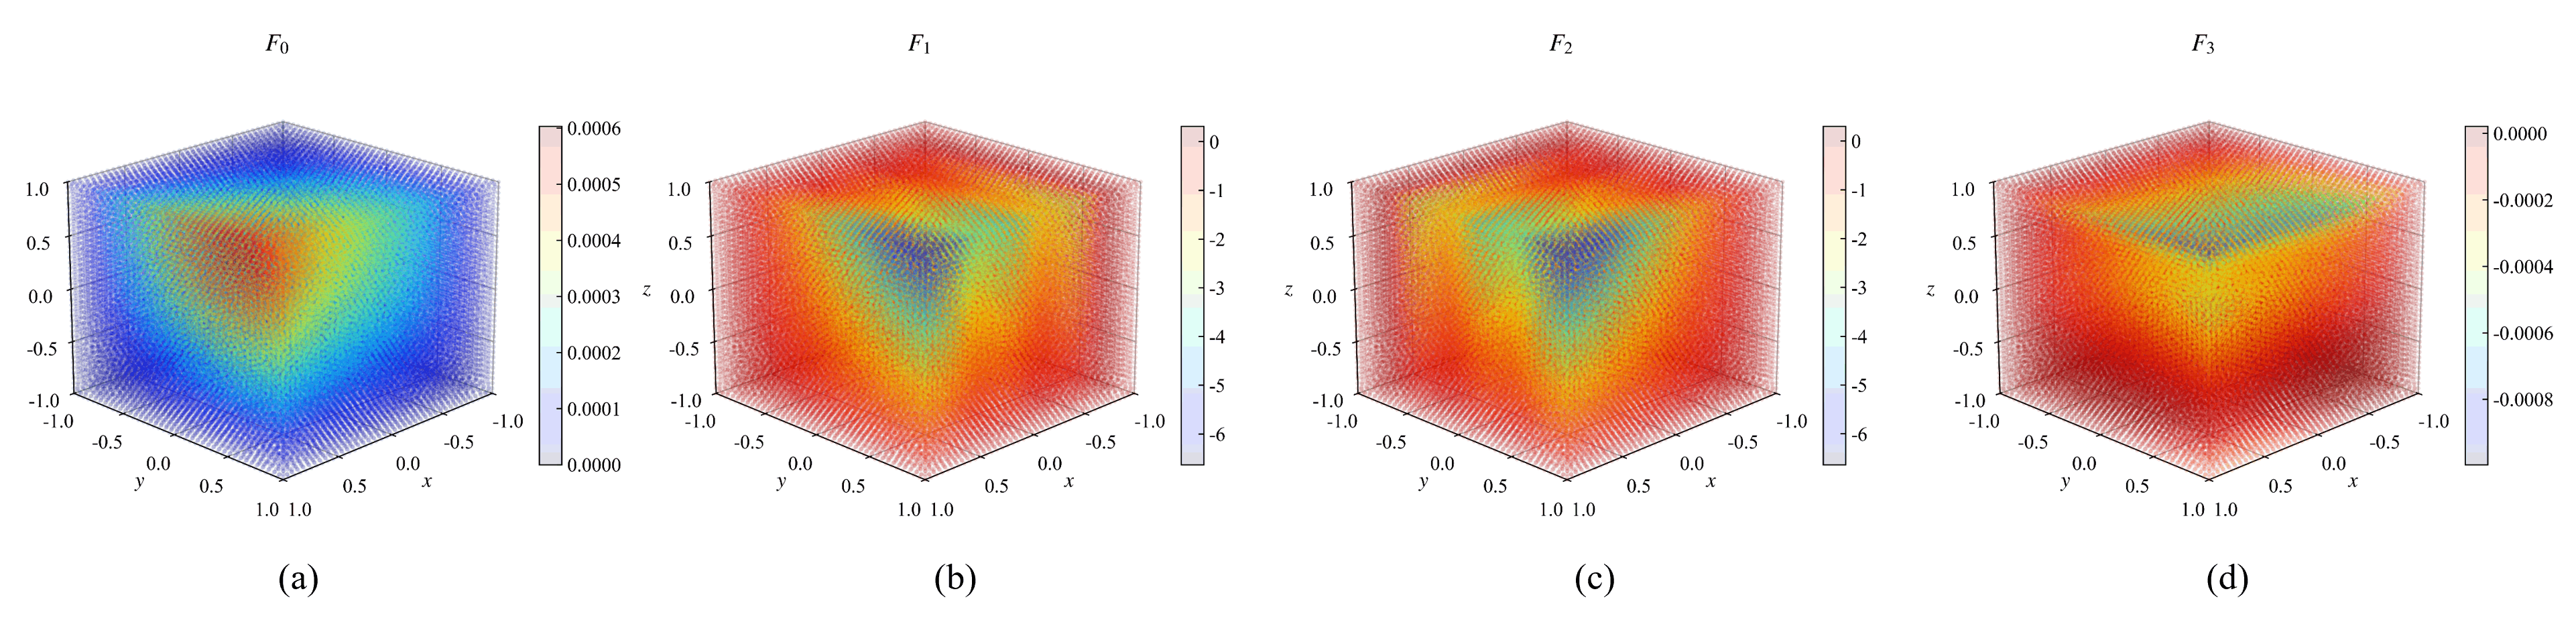
\includegraphics[width=1\textwidth]{fig/figure_09.png}
    \caption{Antiderivative fields for the 3D single-group fixed-source problem with a cylindrical rod bundle array. (a) $F_0$; (b) $F_1$; (c) $F_2$; (d) $F_3$.}
    \label{fig:case3_antiderivative_fields}
\end{figure}

The results show that VIWS can effectively solve high-dimensional interface problems with complex geometries and can also handle mixed Dirichlet and Neumann boundary conditions.

%=============================================================
\subsection{2D two-group fixed-source problem in an L-shaped domain}
\label{subsec:case4}

This example further considers a two-group coupled fixed-source problem in an irregular geometry. The fast-group and thermal-group fluxes are denoted by $\phi_1$ and $\phi_2$, respectively, and the spatial coordinate is $\boldsymbol r=(x,y)$. The governing equations are
\begin{equation}
    \begin{aligned}
        -\nabla \cdot \left( D_1 \nabla \phi_1(\boldsymbol r) \right)
        +\left(\Sigma_{\mathrm a,1} + \Sigma_{\mathrm s,1\rightarrow2}\right)\phi_1(\boldsymbol r)
         & =
        \nu_{1}\Sigma_{\mathrm f,1}\phi_1(\boldsymbol r)
        +\nu_{2}\Sigma_{\mathrm f,2}\phi_2(\boldsymbol r)
        +S_1(\boldsymbol r), \\
        -\nabla \cdot \left( D_2 \nabla \phi_2(\boldsymbol r) \right)
        +\Sigma_{\mathrm a,2}\phi_2(\boldsymbol r)
         & =
        \Sigma_{\mathrm s,1\rightarrow2}\phi_1(\boldsymbol r)
        +S_2(\boldsymbol r).
    \end{aligned}
    \label{eq:case4}
\end{equation}

The computational domain is a two-dimensional L-shaped region, which consists of three material subdomains $\Omega_1$, $\Omega_2$, and $\Omega_3$. \cref{fig:case4_geometry_reference}(a) shows the geometry and material regions, and \cref{fig:case4_geometry_reference}(b) and \cref{fig:case4_geometry_reference}(c) show the FEM reference fluxes of the fast group and thermal group, respectively. The two-group material parameters are listed in \cref{tab:case4_material_parameters}.

\begin{table}[H]
    \centering
    \small
    \caption{Material parameters for the 2D two-group fixed-source problem in an L-shaped domain}
    \label{tab:case4_material_parameters}
    \begin{tabularx}{0.95\textwidth}{@{\extracolsep{\fill}}ccccccc}
        \toprule
        Subdomain
         & Group
         & $D_g$ (cm)
         & $\Sigma_{\mathrm a,g}$ (cm$^{-1}$)
         & $\nu_g\Sigma_{\mathrm f,g}$ (cm$^{-1}$)
         & $\Sigma_{\mathrm s,1\rightarrow2}$ (cm$^{-1}$)
         & $S_g$ (cm$^{-3}\cdot$s$^{-1}$)                                                                                      \\
        \midrule
        $\Omega_1$
         & 1                                              & 1.255  & 0.013052 & 0.00480 & 0.02533 & 1 \\
         & 2                                              & 0.2110 & 0.10030  & 0.00000 &         & 0 \\

        $\Omega_2$
         & 1                                              & 1.268  & 0.011501 & 0.00432 & 0.02767 & 0 \\
         & 2                                              & 0.1902 & 0.07047  & 0.00000 &         & 0 \\

        $\Omega_3$
         & 1                                              & 1.259  & 0.012562 & 0.00456 & 0.02617 & 0 \\
         & 2                                              & 0.2091 & 0.08344  & 0.00000 &         & 0 \\
        \bottomrule 
    \end{tabularx}
\end{table}

\begin{figure}[H]
    \centering
    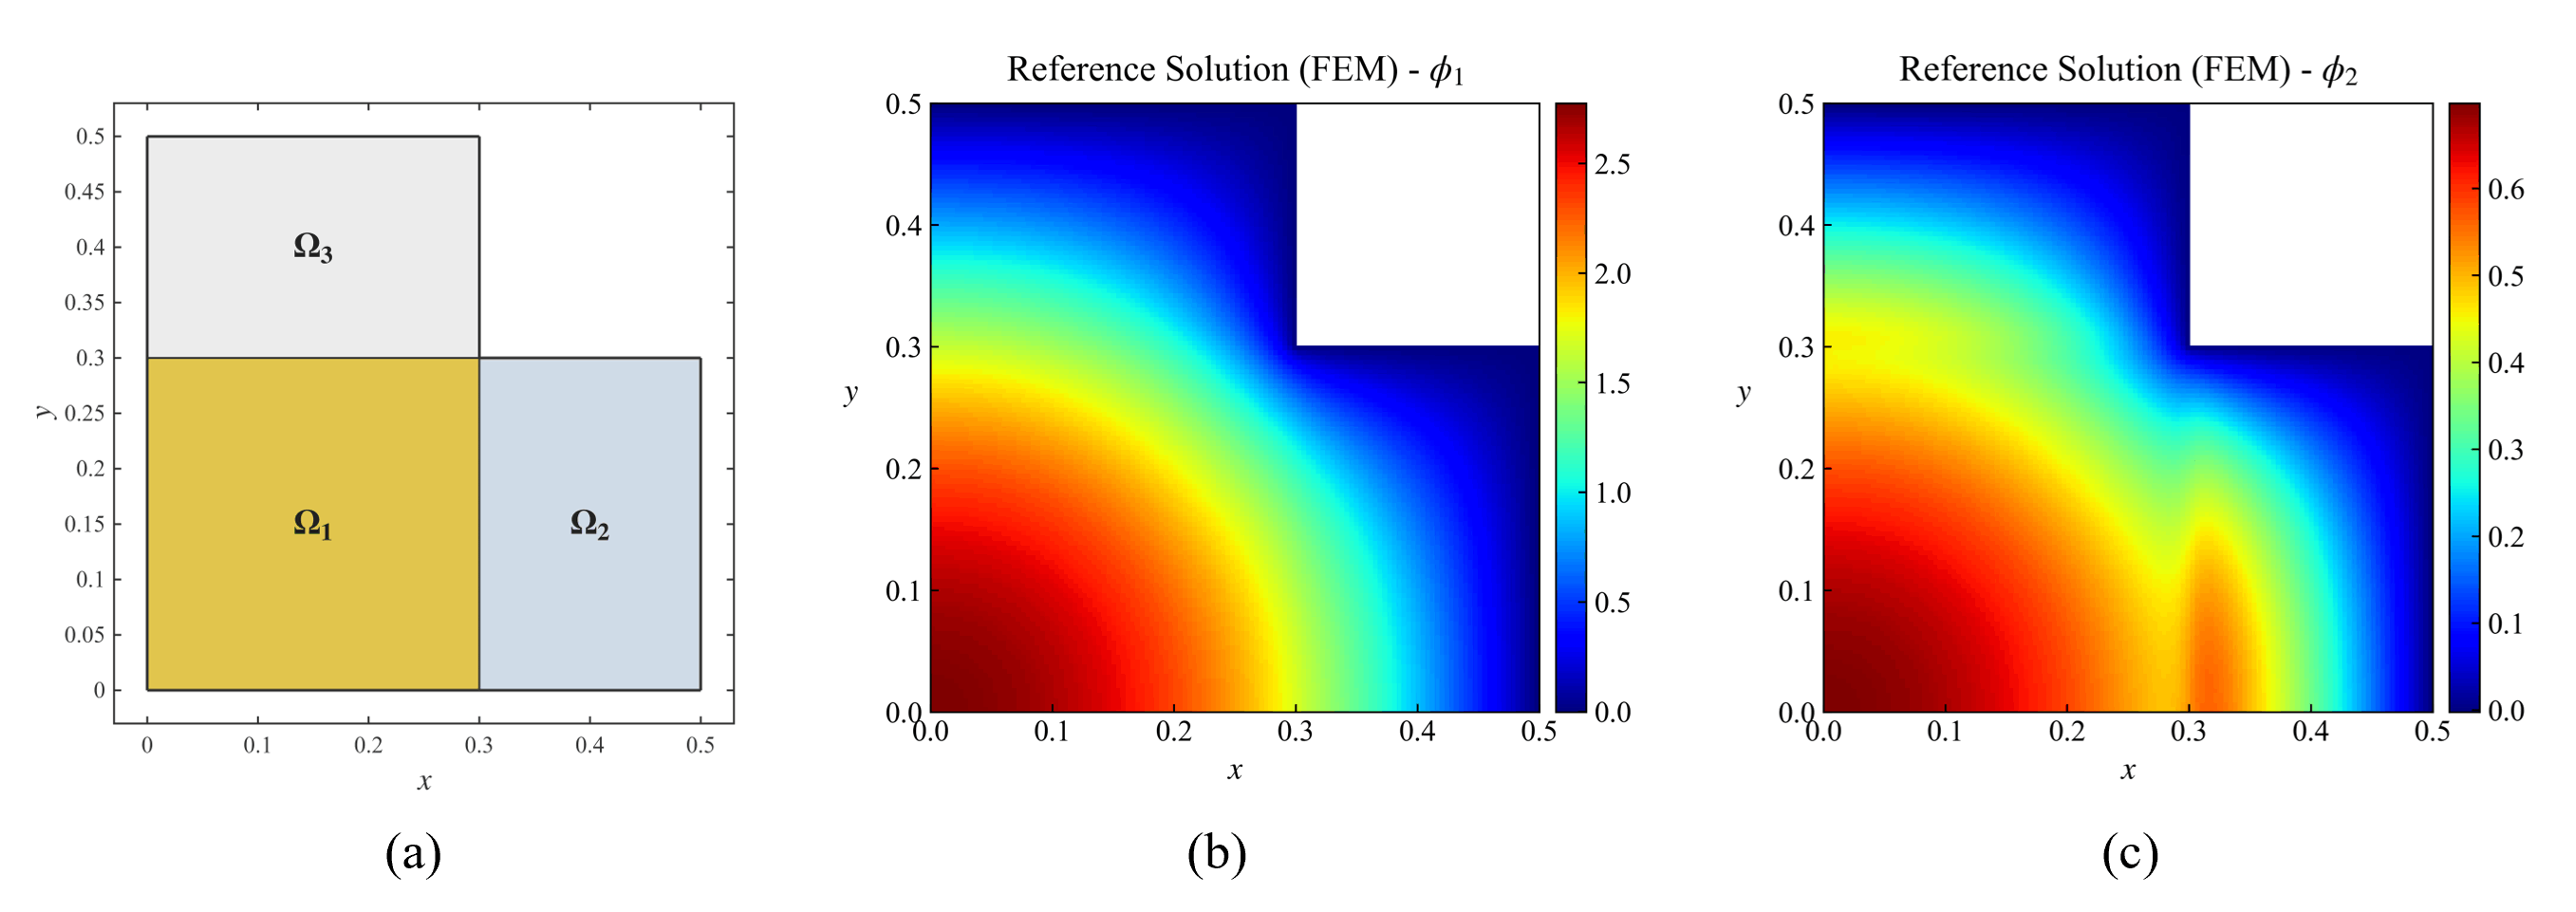
\includegraphics[width=0.75\textwidth]{fig/figure_10.png}
    \caption{Computational setup of the 2D two-group fixed-source problem in an L-shaped domain. (a) Geometry and material regions; (b) FEM reference flux of the fast group; (c) FEM reference flux of the thermal group.}
    \label{fig:case4_geometry_reference}
\end{figure}

Zero-flux Dirichlet conditions are imposed on the right and top boundaries, and zero-normal-current Neumann conditions are imposed on the left and bottom boundaries:
\begin{equation}
    \begin{aligned}
        \phi_g(\boldsymbol r)                         & = 0,
                                                      &      & \boldsymbol r\in\partial\Omega_{\mathrm D}, \\
        \nabla\phi_g(\boldsymbol r)\cdot\boldsymbol n & = 0,
                                                      &      & \boldsymbol r\in\partial\Omega_{\mathrm N},
    \end{aligned}
    \qquad g=1,2 ,
    \label{eq:case4_bc}
\end{equation}
where $\boldsymbol n$ is the outward unit normal vector, and $\partial\Omega_{\mathrm D}$ and $\partial\Omega_{\mathrm N}$ denote the Dirichlet boundary and the Neumann boundary, respectively.

In this example, two independent neural networks are used to represent $\phi_1$ and $\phi_2$, respectively. The test function is chosen as $v=x+y+1$, and $13{,}783$ points are uniformly sampled in the domain. \cref{fig:case4_flux_error_comparison} shows the VIWS predictions and absolute errors for the fast-group and thermal-group fluxes. The relative $L_2$ errors of the fast group and thermal group are
$\epsilon_{L_2}^{(1)}=4.66\times10^{-3}$ and
$\epsilon_{L_2}^{(2)}=2.10\times10^{-2}$, respectively. The larger errors are mainly located near the re-entrant corner of the L-shaped domain. The results show that VIWS can handle two-group coupled fixed-source problems in irregular geometries.

\begin{figure}[H]
    \centering
    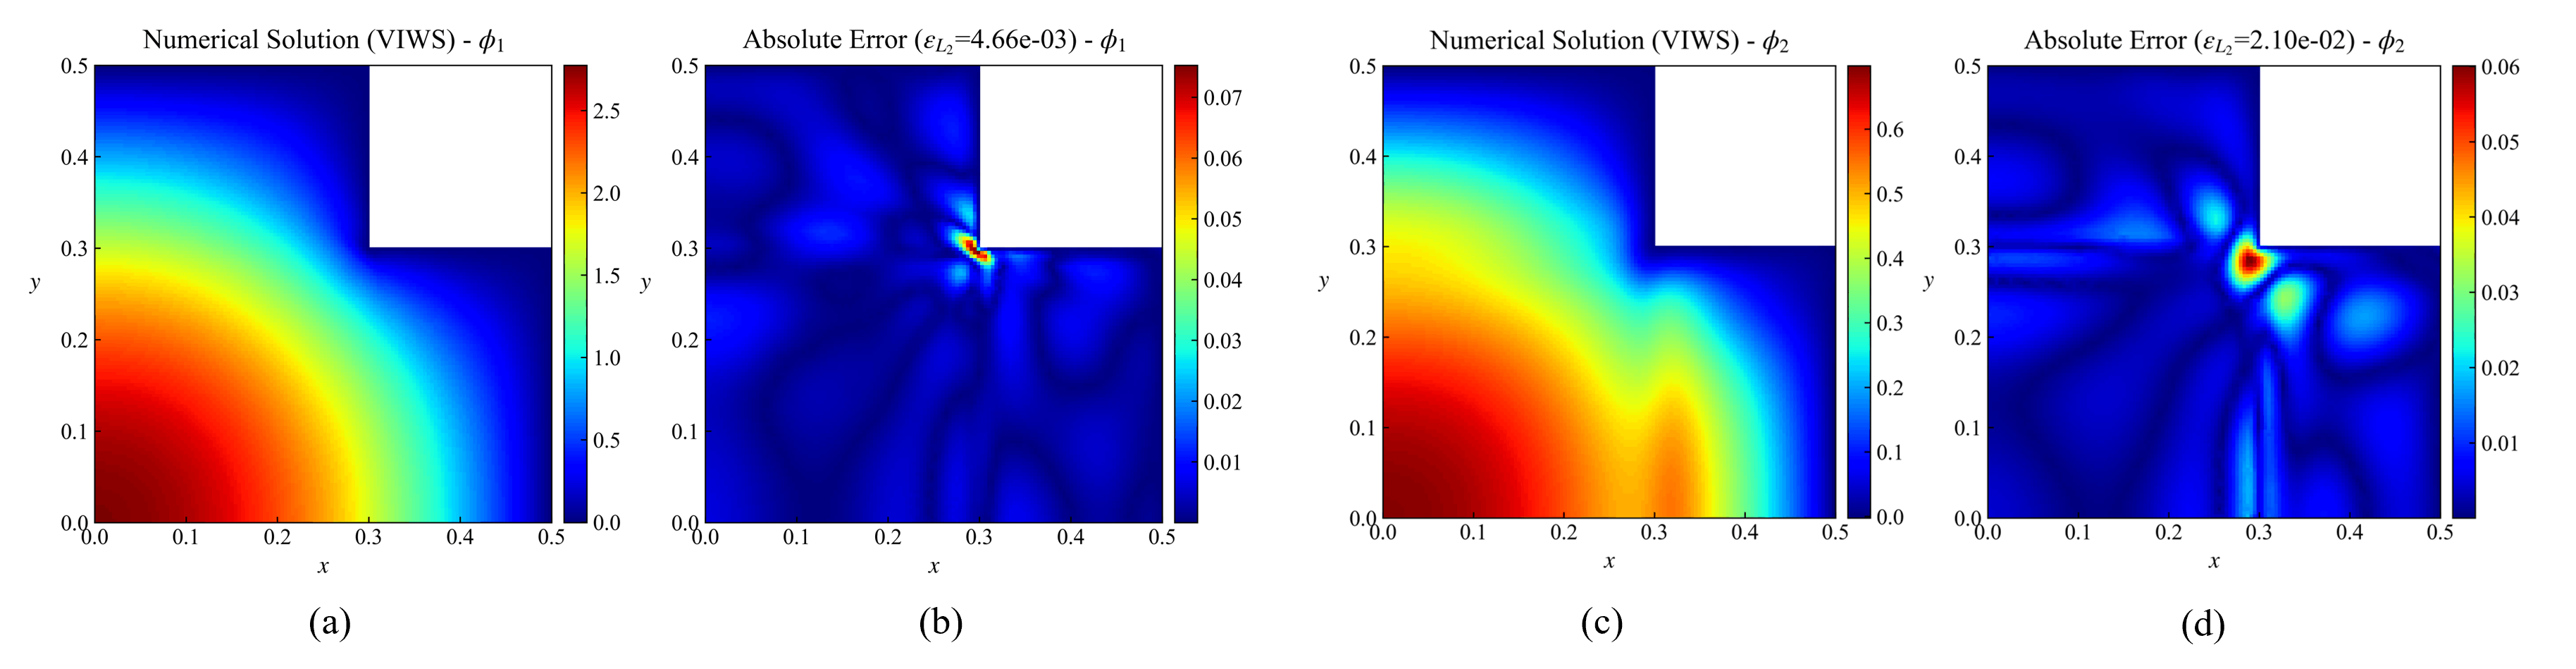
\includegraphics[width=1\textwidth]{fig/figure_11.png}
    \caption{VIWS flux prediction and error distribution for the 2D two-group fixed-source problem in an L-shaped domain. (a) Predicted fast-group flux; (b) absolute error of the fast group; (c) predicted thermal-group flux; (d) absolute error of the thermal group.}
    \label{fig:case4_flux_error_comparison}
\end{figure}

%=============================================================
\subsection{2D-IAEA two-group neutron diffusion eigenvalue benchmark}
\label{subsec:case5}

This example uses the classical 2D-IAEA pressurized water reactor (PWR) two-group neutron diffusion eigenvalue benchmark. It aims to verify the applicability of the VIWS framework to complex multi-material geometries and eigenvalue problems. This problem neglects the effect of delayed neutron precursors~\cite{theler2011solution}. Its governing equations and the corresponding variable-domain integral weak form are given in \cref{eq:two_group_eigenvalue} and \cref{eq:two_group_variable_weak_form}, respectively.

For the core configuration, this benchmark consists of two types of fuel regions and an outer reflector, with a total of 177 fuel assemblies. The width of each assembly is $20,\mathrm{cm}$, and the thickness of the surrounding reflector is also $20,\mathrm{cm}$. Based on the symmetry of the geometry and material distribution, only one-quarter of the domain is used in the calculation. This quarter domain includes four types of material subregions, $\Omega_1$--$\Omega_4$, and their layout is shown in \cref{fig:case5_geometry_reference}(a). The boundary conditions are set as follows: zero-normal-current Neumann conditions are used on the symmetry boundaries, and zero-flux Dirichlet conditions are used on the outer boundaries. The related material group constants are listed in \cref{tab:case5_material_parameters}. In addition, \cref{fig:case5_geometry_reference}(b) and (c) show the fast-group and thermal-group reference flux distributions obtained by the finite element method (FEM), respectively. The corresponding reference effective multiplication factor is $k_{\mathrm{eff}}=1.03394$.

The flux magnitude of an eigenvalue problem is not uniquely scaled \cite{liu2022solving}. To fix the eigenfunction amplitude and avoid the trivial solution, a global normalization constraint is imposed on the fast-group flux:
\begin{equation}
    \mathcal{L}_{\mathrm{norm}}
    =
    \left(
    \frac{1}{N_r}
    \sum_{i=1}^{N_r}
    \phi_1^2(\boldsymbol r_i)
    -1
    \right)^2 .
    \label{eq:loss_norm}
\end{equation}
At the same time, Fourier feature mapping~\cite{tancik2020fourier} is introduced at the network input to improve the network's ability to represent material interfaces, geometric corners, and local high-gradient regions. The effective multiplication factor $k_{\mathrm{eff}}$ is treated as a global parameter to be optimized and is updated together with the neural network weights \cite{liu2023deep}. A total of $54,677$ points are uniformly sampled in the domain, and the test function is chosen as $v=1$.
\begin{table}[H]
\centering
\small
\caption{Material parameters for the 2D-IAEA two-group neutron diffusion eigenvalue benchmark}
\label{tab:case5_material_parameters}
\begin{tabularx}{0.95\textwidth}{@{\extracolsep{\fill}}ccccccc}
\toprule
Subdomain
& Group
& $D_g$ (cm)
& $\Sigma_{\mathrm a,g}$ (cm$^{-1}$)
& $\nu_g \Sigma_{\mathrm f,g}$ (cm$^{-1}$)
& $\Sigma_{\mathrm s,1\rightarrow2}$ (cm$^{-1}$)
& Material \\
\midrule
$\Omega_1$
& 1 & 1.5 & 0.010 & 0.000 & 0.02 & Fuel 1 \\
& 2 & 0.4 & 0.080 & 0.135 & & \\
$\Omega_2$
& 1 & 1.5 & 0.010 & 0.000 & 0.02 & Fuel 2 \\
& 2 & 0.4 & 0.085 & 0.135 & & \\\
$\Omega_3$
& 1 & 1.5 & 0.010 & 0.000 & 0.02 & Fuel 2 + control rod \\
& 2 & 0.4 & 0.130 & 0.135 & & \\
$\Omega_4$
& 1 & 2.0 & 0.000 & 0.000 & 0.04 & Reflector \\
& 2 & 0.3 & 0.010 & 0.000 & & \\
\bottomrule
\end{tabularx}
\end{table}

\begin{figure}[H]
    \centering
    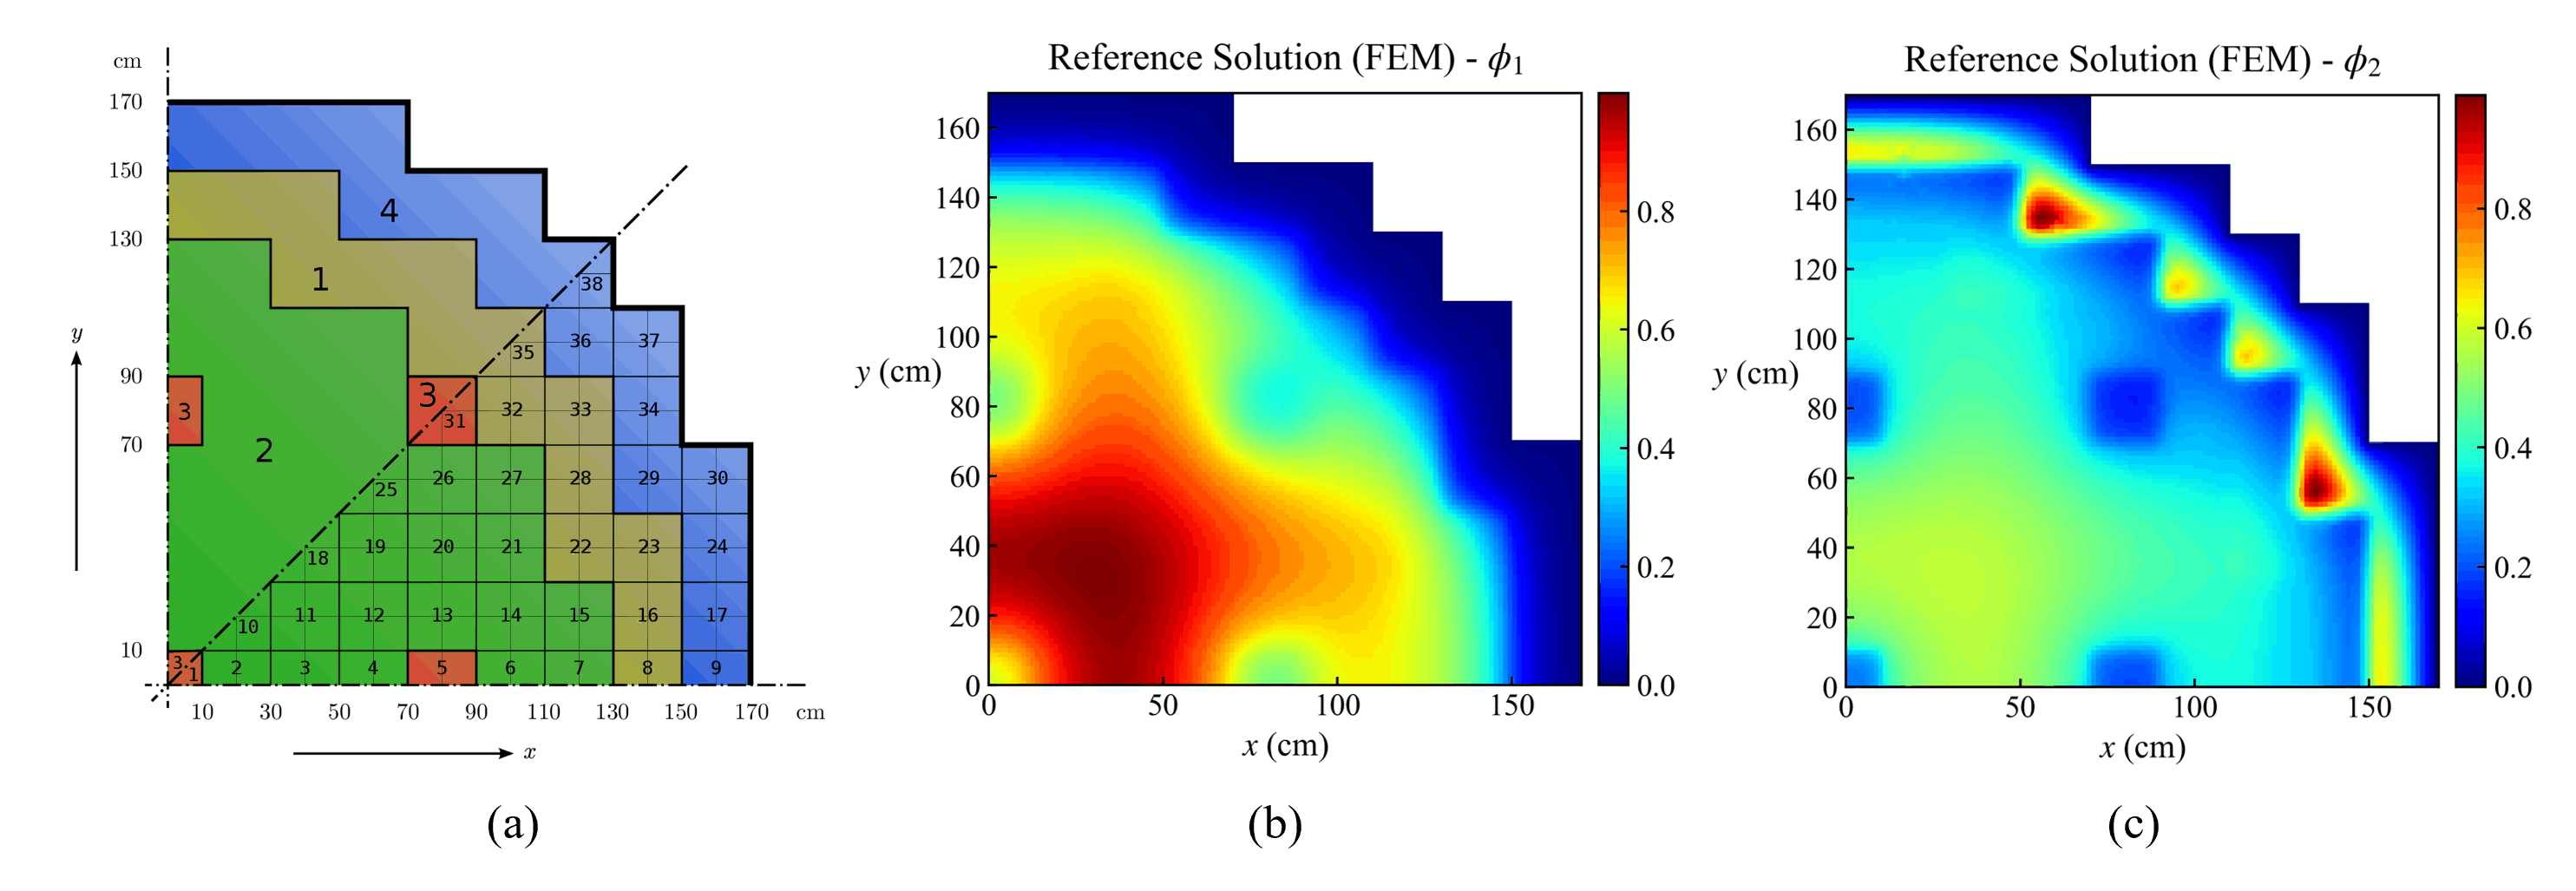
\includegraphics[width=0.75\textwidth]{fig/figure_12.png}
    \caption{Computational setup of the 2D-IAEA two-group neutron diffusion eigenvalue benchmark. (a) Quarter-core geometry and material regions; (b) FEM reference flux of the fast group; (c) FEM reference flux of the thermal group.}
    \label{fig:case5_geometry_reference}
\end{figure}

\begin{figure}[H]
    \centering
    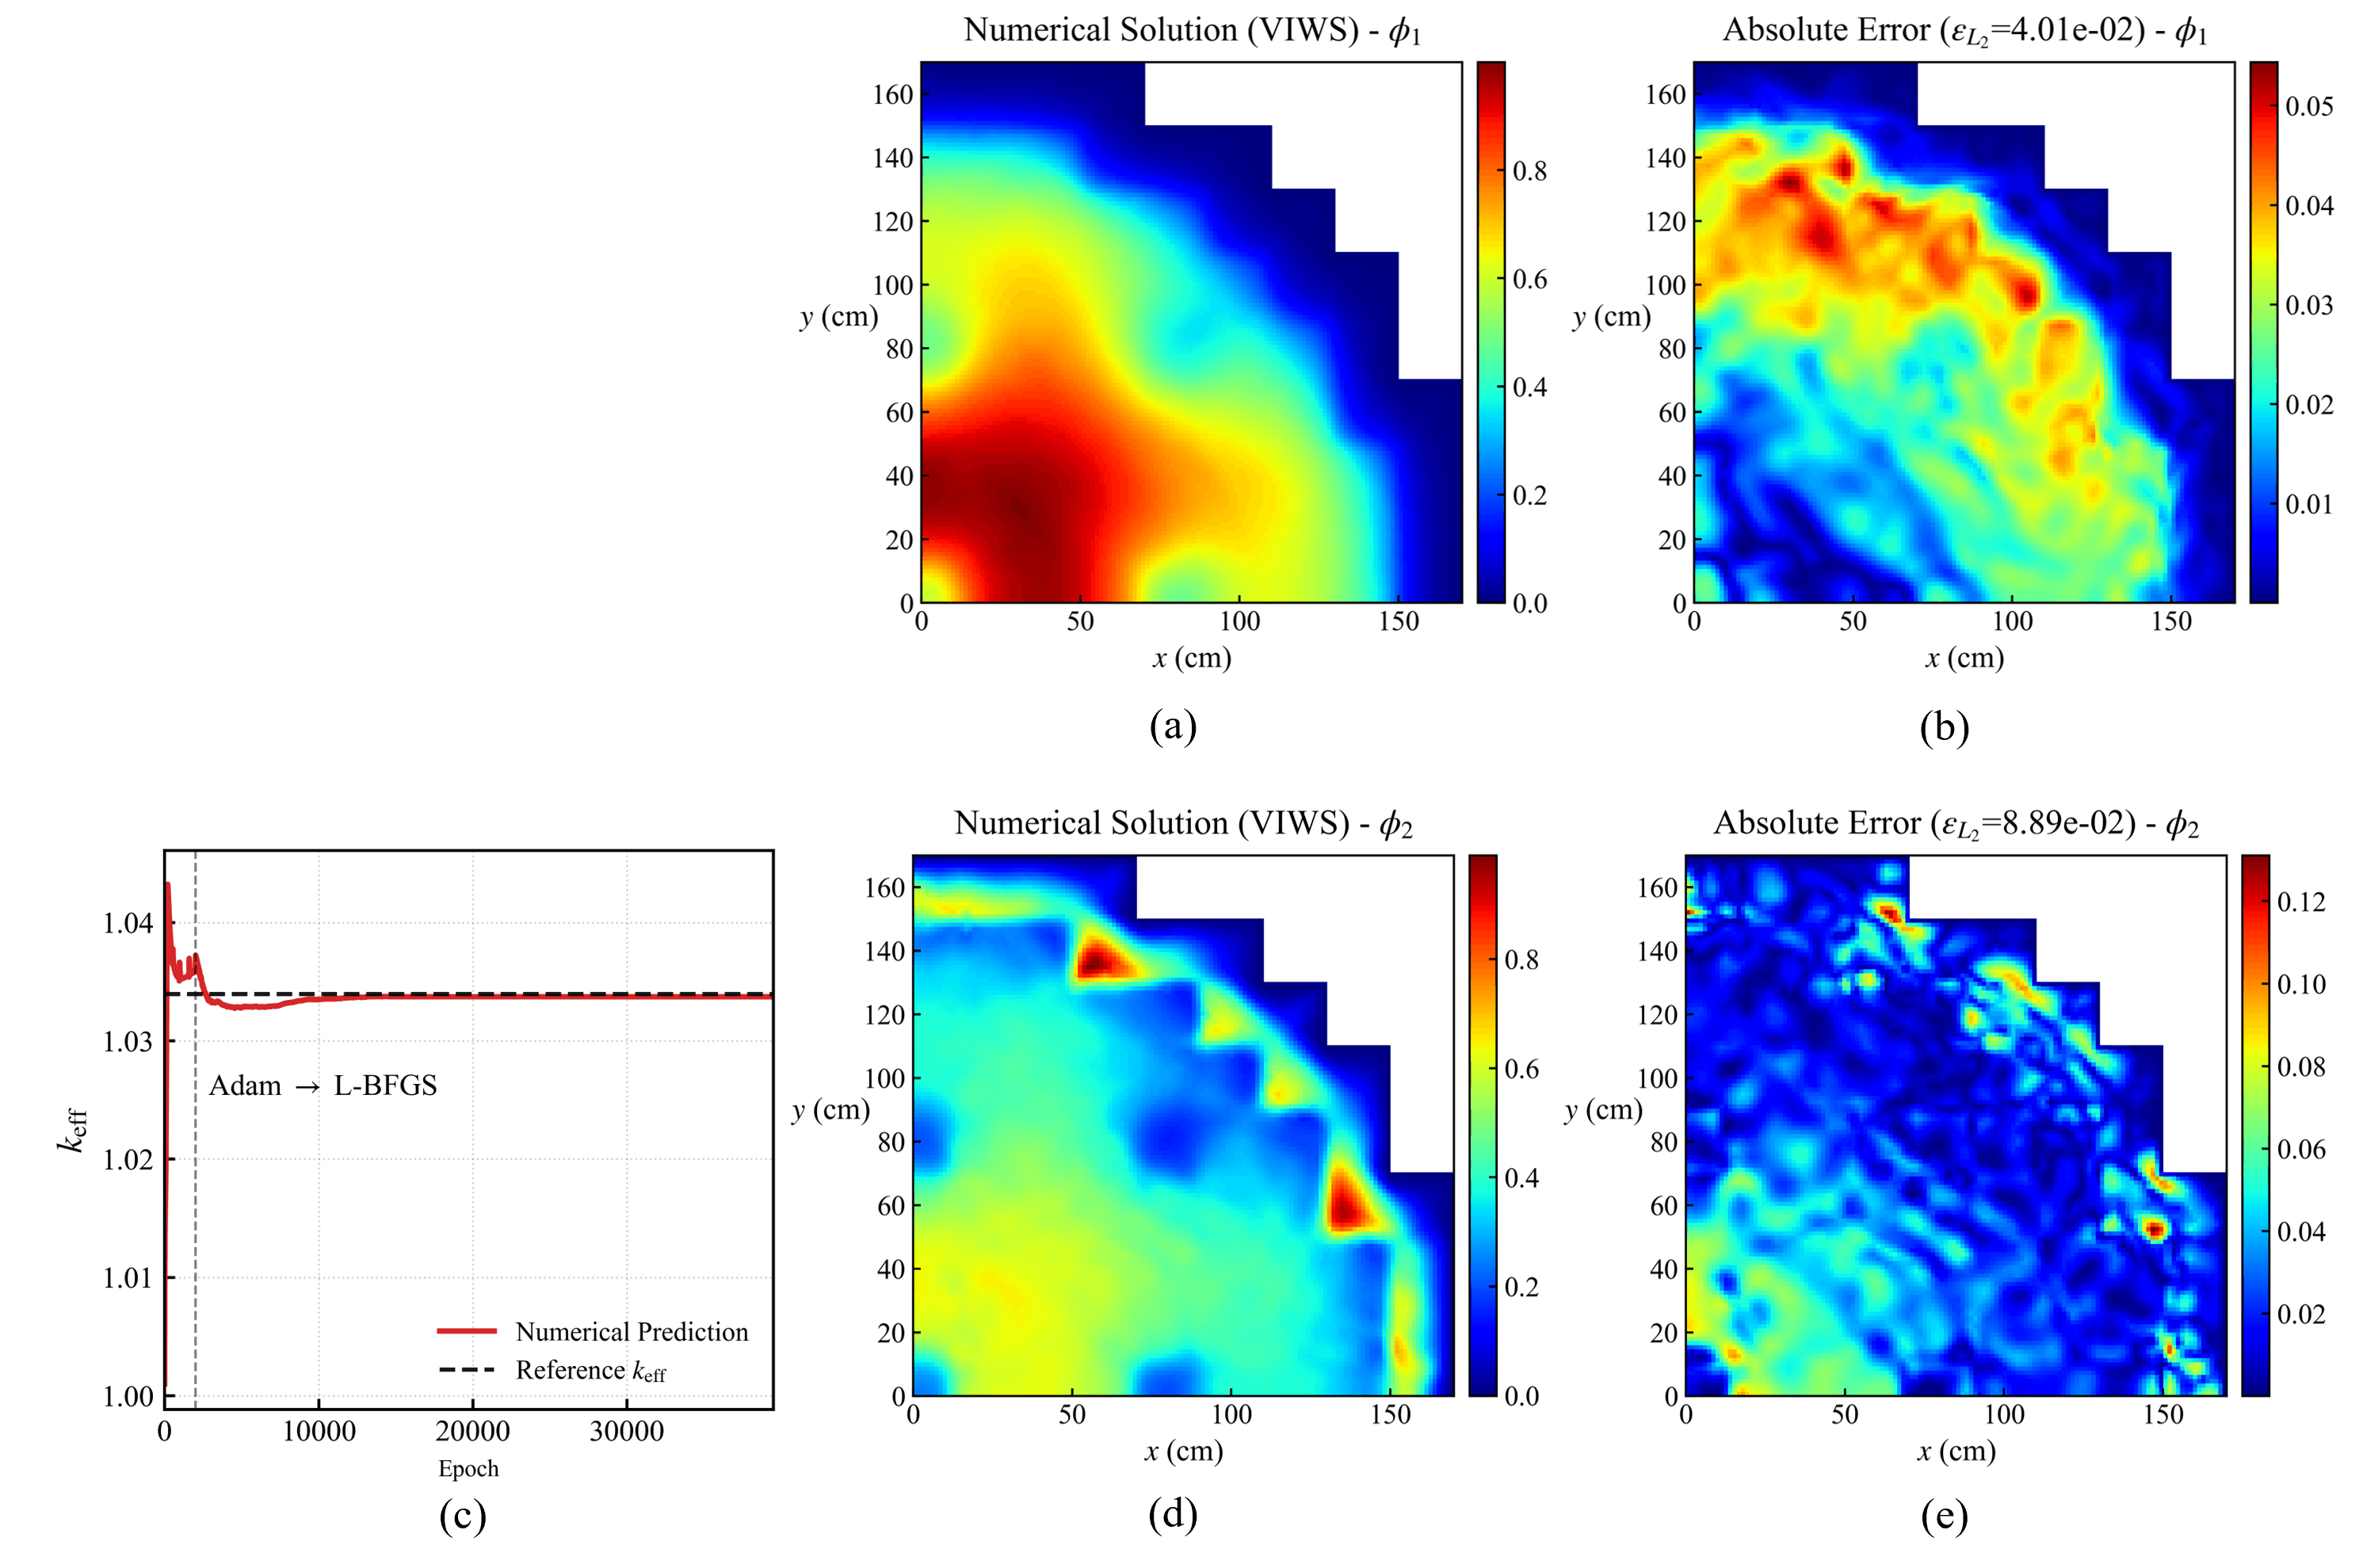
\includegraphics[width=0.75\textwidth]{fig/figure_13.png}
    \caption{VIWS results for the 2D-IAEA two-group neutron diffusion eigenvalue benchmark. (a) Predicted fast-group flux; (b) absolute error of the fast group; (c) convergence curve of $k_{\mathrm{eff}}$; (d) predicted thermal-group flux; (e) absolute error of the thermal group.}
    \label{fig:case5_flux_error_keff}
\end{figure}

\cref{fig:case5_flux_error_keff} shows the two-group flux predictions, error distributions, and the convergence process of $k_{\mathrm{eff}}$ obtained by VIWS. The computed result is $k_{\mathrm{eff}}=1.03372$, with a deviation of approximately $22$ pcm from the FEM reference value. The relative $L_2$ errors of the fast-group and thermal-group fluxes are
$\epsilon_{L_2}^{(1)}=4.01\times10^{-2}$ and
$\epsilon_{L_2}^{(2)}=8.89\times10^{-2}$, respectively. 
The results show that VIWS can be used for two-group neutron diffusion eigenvalue problems with engineering-type geometries, and it can provide both the effective multiplication factor and the corresponding flux fields.

\section{Conclusion}
\label{sec:conclusion}

This paper applies the variable-domain integral weak solution (VIWS) theory to deep learning-based neutron diffusion calculations in heterogeneous media. The main contributions are summarized as follows. First, variable-domain integration regions are introduced into the integration-by-parts process, a VIWS form of the neutron diffusion equation is constructed for complex geometries and multigroup conditions. This form effectively reduces the difficulty caused by interface derivative singularities in solving neutron diffusion equations and improves the calculation accuracy. Second, a single-network framework is used to represent the global numerical solution of the neutron diffusion equation. Based on the principle of flux continuity, the interface derivative jumps are handled implicitly, avoiding the explicit treatment of complex internal interface conditions. Finally, for integral terms with continuous kernels, they are further transformed into the corresponding antiderivative forms and used in the deep learning solution, which improves computational efficiency.

The numerical results show that the proposed method has high accuracy in solving two-dimensional and three-dimensional neutron diffusion problems in heterogeneous media, and is significantly better than the classical PINN method. It is applicable to irregular boundaries, mixed boundary conditions, multigroup coupling, and eigenvalue calculation, and shows potential for further engineering-oriented applications.

Future work may focus on extending the proposed method to practical applications such as three-dimensional space-time neutron kinetics problems, multiphysics coupling, and large-scale complex reactor core problems. In addition, future studies may combine the method with new neural network architectures and machine learning methods based on large-scale parallel computing, so as to further improve the accuracy and efficiency of deep learning methods in neutron diffusion calculation and promote practical engineering applications.

\section*{Acknowledgments}

This research is supported by the National Natural Science Foundation of China (Grant No. 12575189), the Basic Research and Stable Support Research Project of Science and Technology Industry Bureau of China (Grant No. WDZC2023050305), the Sichuan Science and Technology Program (Grant No. 2023YFG0373), and the National Defense Basic Scientific Research Program of China (Grant No. JCKY2024110C080).

% \newpage
\bibliographystyle{elsarticle-num}
\bibliography{C:/Users/mathliuyang/Zotero/ref_BibTeX}

\end{document}

\endinput
%%
%% End of file `main.tex'.
